\chapter{Background theory}\label{chapter:theory}

This chapter gives an overview of some of the most important strategies for terrestrial snake robot locomotion to address the first part of the thesis project description. The rest of the chapter focuses on theory required to adapt the method of dynamic HPFC to the snake robot model. This includes an explanation of the snake robot kinematics, dynamics and constraints.

%Lastly, both "traditional" HPFC and dynamic HPFC is explained in detail and discussed with regard to the snake robot application.

Some parts of this chapter are fully or partly taken from the previous project work of the author \cite{AtussaProsjektoppgp}. This is stated in the respective sections.


\section{Terrestrial snake robot locomotion strategies}\label{sec:locomotion}


%--------------------------------------------------------------------------
%--------------------------------------------------------------------------

Several methods have been proposed for snake robot locomotion, most of which are inspired by nature. This part presents some of the well established strategies, as well as the newer approach, obstacle aided locomotion, which this report is based on. Finally, compliance control in snake robot locomotion is presented to open up for a comparison to what the hybrid position/force control offers.

\subsection{Traditional locomotion strategies}\label{subsec:traditional-loco}

\textbf{Lateral undulation} is the fastest and by far the most commonly implemented locomotion gait for snake robots \cite{sanfilippo2017perception}.
It is a continuous movement of the entire body of the snake relative to the ground. The locomotion is obtained by propagating sine-waves from the front to the rear of the snake \cite{transeth2006developments}, as illustrated in figure \ref{fig:lateral}.
Successful propulsion by lateral undulation requires that the snake has some grip to the surface enabling it to glide forward without slipping sideways \cite{liljeback2012review}. This again puts requirements on the friction coefficients, namely that the coefficient in lateral direction have to be greater than in the forward
direction. If the movement is conducted without slipping, every part of the body will pass through the same points on the ground.

\textbf{Concertina locomotion} is not employed on open ground, but rather in narrow spaces where the available range of motion is limited. The motion is carried out by curving the body
to create an anchor against the narrow environment (see figure \ref{fig:concertina}). The snake alternates between curving the back and front part of the body so that the front part can be stretched forward and the back part can be drawn up \cite{liljeback2012snake}.

A resembling mode of locomotion is \textbf{sidewinding}, in which one part of the body acts as an anchor while the other part is moved forward. The part that moves forward is simply lifted off the ground and displaced while the other part stays put, typically in areas with loose sand \cite{liljeback2012snake}. It can be seen as a kind of spiraling motion. Figure \ref{fig:sidewinding} gives a visual explanation of this gait.


% Rectlinear crawling?

\begin{figure}[H]
    \centering
    
    \subfloat[Lateral undulation \label{fig:lateral}]{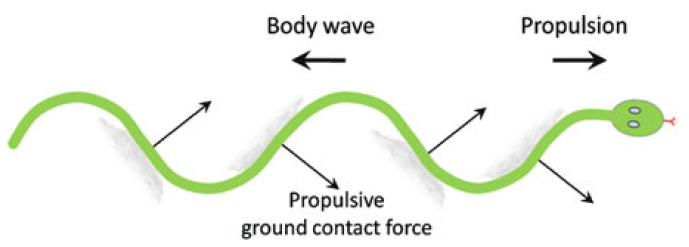
\includegraphics[clip=true, width=0.6\textwidth]{figures/theory/lateral.PNG}}

    \subfloat[Concertina locomotion \label{fig:concertina}]{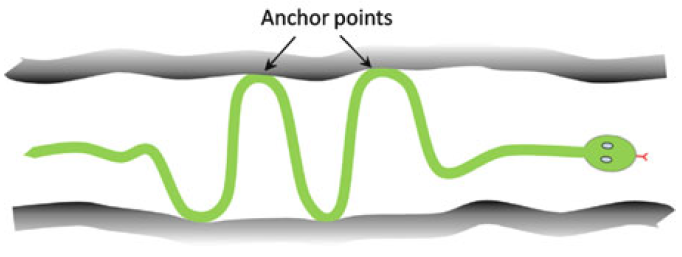
\includegraphics[clip=true, width=0.6\textwidth]{figures/theory/concertina.PNG}}

   \subfloat[Sidewinding \label{fig:sidewinding}]{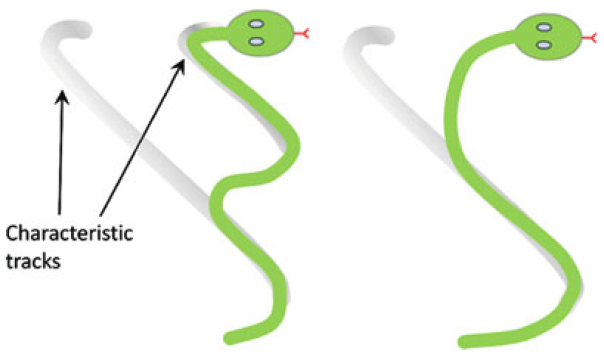
\includegraphics[clip=true, width=0.6\textwidth]{figures/theory/Sidewinding.PNG}}

    \caption{Illustration of some traditional locomotion strategies \cite{liljeback2012snake}.}
    \label{fig:traditional_locomotion}
\end{figure}


\subsection{Central pattern generators (CPGs)}

The information presented in this section is taken from \cite{ijspeert2008central}.

A central pattern generator for locomotion control is where neuroscience meets robotics. CPGs consist of neurons that produce an oscillating, rhythmic output without requiring sensory information. In nature, CPGs play an important role in periodic actions like breathing, walking and other modes of locomotion. While sensory feedback is not needed for generating the rhythms, it plays a very important role in shaping the rhythmic patterns. This is fundamental for keeping CPGs and body movements coordinated.

The method produces stable rhythmic patterns and is able to rapidly return the system to its normal rhythmic behavior after transient perturbations. Furthermore, CPG models tend to reduce the dimensionality/complexity of the control problem in that they have only a few control parameters. These parameters allow modulation of the locomotion, for instance the speed and direction or even the type of gait. This allows for higher-level controllers to circumvent the generation of multidimensional motor commands and stick to higher level control signals.

CPGs can be applied to cyclic locomotion gaits like lateral undulation, sidewinding and concertina locomotion since they are based on rhythmic patterns.

\subsection{Obstacle-aided locomotion (OAL)}\label{subsec:OAL}

Aforementioned locomotion strategies are first and foremost successful in plain, obstacle-free environments where ground friction can be used to achieve propulsion. The OAL method, on the other hand, considers flat environments with obstacles. The obstacles can be compared to the ground friction in other locomotion gaits like lateral undulation. This is because both obstacles and ground friction are used to push against. Thus, OAL can be seen as a kind of discrete special case of lateral undulation. The rest of the explanation of OAL is taken from the project work of the author \cite{AtussaProsjektoppgp}.

Instead of avoiding physical contact between the robot and obstacles, obstacle aided locomotion aims at profiting from it by using the obstacles as push-points to propel itself forward. This concept is illustrated in Figure \ref{fig:oal}. OAL was first introduced by Transeth et al. in 2008 \cite{transeth2008snake}. The motivation behind this method was based in the ability of biological snakes to utilize irregularities in the terrain for more efficient locomotion.

Liljebäck et al. \cite{liljeback2012snake} describe two major challenges related to OAL:
\begin{enumerate}
  \item It is unknown in advance when and where the snake robot will make contact with its environment.
  \item The development of a strategy for adjusting the shape of the robot so that forward propulsion is achieved in any given contact situation.
\end{enumerate}
The following hypothesis is also stated in \cite{liljeback2012snake}.
\begin{quote}
   \textit{ Obstacle-aided snake robot locomotion can be achieved by producing body shape changes where the links in contact with obstacles are rotated so that the components of the contact forces in the desired direction of motion are increased.}
\end{quote}

Holden et al. \cite{holden2014optimal} address the second challenge by formulating an optimization problem that seeks to minimize energy consumption while achieving propulsion along a user-defined desired path. The output of this optimization is the optimal motor torque inputs. In addition to a user-defined path, this method assumes that the desired link angles at the obstacles are given.

Bayraktaroglu et al. \cite{bayraktaroglu2004understanding} mention that only the trajectory of the leading link should be arbitrarily determined. Moreover, Bayraktaroglu et al. \cite{bayraktaroglu2004understanding} state that in a steady smooth motion, the trajectory of the leading link must be computed as a function of available push-points for the next contact, and the desired position and orientation of the following links are those that mimic the motion of the leading link.

\begin{figure}
    \centering
    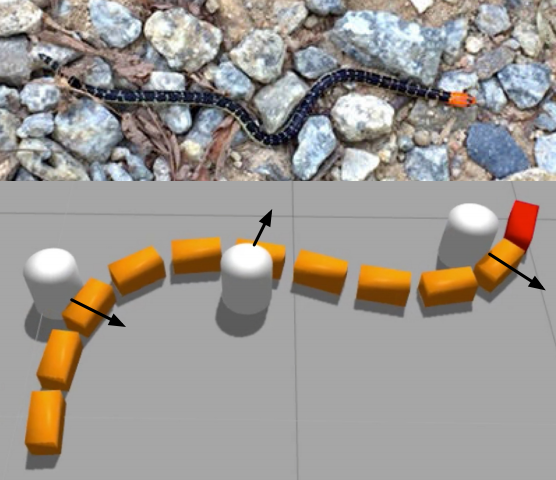
\includegraphics[width=0.6\textwidth]{figures/theory/oal.PNG}
    \caption{Obstacle-aided locomotion illustration \cite{sanfilippo2017snakesim}}
    \label{fig:oal}
\end{figure}

%--------------------------------------------------------------------------
%--------------------------------------------------------------------------


\subsection{Locomotion strategies with compliance control}\label{subsec:compliance-control}

Biological snakes cannot in any way be seen as rigid animals. Robots, on the other hand, are by default very rigid, both in the body material and actuators used.
Compliant control is fundamental when dealing with unstructured environments because it implicitly controls the energy transfer to the environment \cite{calanca2015review}.

Two main methods can be applied to snake robots to mimic the compliant and adaptive behavior between snakes and the environment they traverse. The first method is using a compliant controller for the actuators, in which they adapt a spring-like behavior. The shape-based compliance and directional compliance, among others, go under this category and are explained here. The second method is directly designing the robot with compliance, meaning that the mechanical parts are compliant.

\subsubsection{Shape-based compliance}

A very common way of controlling the shape of snake robots has been specifying the motion of each individual joint directly. This works well as long as the snake robot is traversing a flat surface without obstacles that would lead to great deviations from the planned motion.
In environments with obstacles, on the other hand, Liljebäck et al. \cite{liljeback2014compliant} proposed a specification of the motion of the robot in terms of \textit{shape control points (SCPs)}. These points specify which coordinates it is desired that the snake goes through. The points are further connected with a shape curve defined by an interpolation technique. The desired joint angles of the snake robot are eventually found by aligning a virtual robot with the shape curve and adapt its joint angles.

The work of \cite{liljeback2014compliant} is based on a model of the snake robot crawling by lateral undulation on a flat surface with circular obstacles. The compliant behavior of the snake robot is then achieved by assigning mass-spring-damper dynamics to the SCPs, making the SCPs and thus the shape curve compliant. \cite{liljeback2014compliant} propose that the adaptive behavior of the shape curve should depend on the direction of the contact force with respect to the forward direction of motion. Consequently, a natural choice is to make the shape curve highly compliant for obstructive contact forces and less compliant for propulsive contact forces.

%\subsubsection{Gait-based compliance}

%Rollinson et al. \cite{rollinson2013gait} proposed a controller in which individual joints can comply to a high-level controller built around gait parameters that specify whole-body motions. The controller is simply commanding an amplitude with a constant offset from the estimated amplitude. In the case which \cite{rollinson2013gait} call "position compliance", a positive offset causes the robot to drive forward in the gait cycle, while a negative offset causes it to drive backwards. Furthermore, the magnitude of the offset determines how hard the robot tries to push forward or backward.

\subsubsection{Directional compliance}

The disadvantage of shape-based compliance is that not all terrain features are helpful for locomotion. Some might impede the movement of the robot instead of aiding it. Because of this, a novel approach called directional compliance has been proposed by Wang et al. \cite{wang2020directional}. The approach is an improved version of the shape-based compliance controller that adapts the compliance according to the information it has about the obstacles. This information is obtained from the force measured through the joints of the robot. Thus, it is what can be called a reactive controller. Directional compliance allows the robot to selectively admit forces applied on one side and reject forces from the other side \cite{wang2020directional}.

The most substantial discovery of Wang et al. \cite{wang2020directional} is that the amplitude of the shape parameters act as an indication of the robot's forward progression. Thus, the amplitude difference from the nominal value is used to determine whether the robot should increase or decrease it's curvature at certain segments of its body. Wang et al. \cite{wang2020directional} denote admitting external forces that result in increases in curvature as positive directional compliance and admitting forces that result in decreases in curvature as negative directional compliance. The known shape-based compliance is the nominal compliance of the controller. Furthermore, a filter function is used to adapt this nominal compliance and include the two other modes.

In summary, directional compliance enables the robot to either push away from, or comply to, terrain features, based on the torque feedback measured over time \cite{wang2020directional}. This dynamical system strategy was proven successful even in a three dimensional environment. However, the main aim of this controller is utilizing obstacles the snake robot "by chance" collides with in order to avoid getting stuck between obstacles, rather than following a specific path. This means that the method is unlikely to choose the most optimal path to move forward, as is desired in OAL.


\subsubsection{Mechanical compliance}

When a robot is mechanically compliant, it typically means that it has flexible or soft mechanics. Several technologies have been explored to realise this property, like pneumatic, hydraulic, polymers etc. \cite{calanca2015review}. According to Calanca \cite{calanca2015review}, most of the implementations at the current state of the art make use of traditional electric motors with the addition of a soft element and/or a compliant controller.

Mechanical compliance allows for implicitly controlling the power transferred to the environment and to exhibit displacement if a force is applied. Furthermore, it is obvious that the response time of a mechanical compliant system always will be faster than a system with a compliant controller. The relation of compliance control to position and force control, is that an ideal position controlled system has zero compliance whilst an ideal force controlled system has infinite compliance \cite{calanca2015review}. 

\clearpage
%--------------------------------------------------------------------------
%--------------------------------------------------------------------------



\section{Snake robot kinematics}\label{sec:kin}


The snake robot is modeled as a serial chain, which is a system of rigid bodies in which each member is connected to two others, except for the first and last members that are each connected to only one other member \cite{waldron2016kinematics}. As opposed to traditional robot manipulator models, the first joint in the snake robot model is not physically connected to a base.


The vector of generalized coordinates $\mathbf{q}$ for a snake robot with $n$ links is

\begin{equation} \label{eq:q}
    \mathbf{q} = 
    \begin{bmatrix}
        \phi_1 & \phi_2 & ... & \phi_n & x_0 & y_0
    \end{bmatrix}^T.
\end{equation}
\\
The coordinates $(x_0, y_0)$ and $\phi_1$ represent the position and orientation of the tail of the snake robot in reference to the base frame $(x,y)$. These coordinates cannot be directly controlled and will therefore be referred to as virtual coordinates. The generalized coordinates ${\phi_2, ... ,  \phi_n}$, corresponding to the actuated joints, refer to the angle of the following link relative to the preceding link. The number of generalized coordinates including two position coordinates and $n$ joint angles is $N = n+2$.

The model of the snake robot with the named variables are illustrated in Figure \ref{fig:kin_name}. 
\begin{figure}
    \centering
    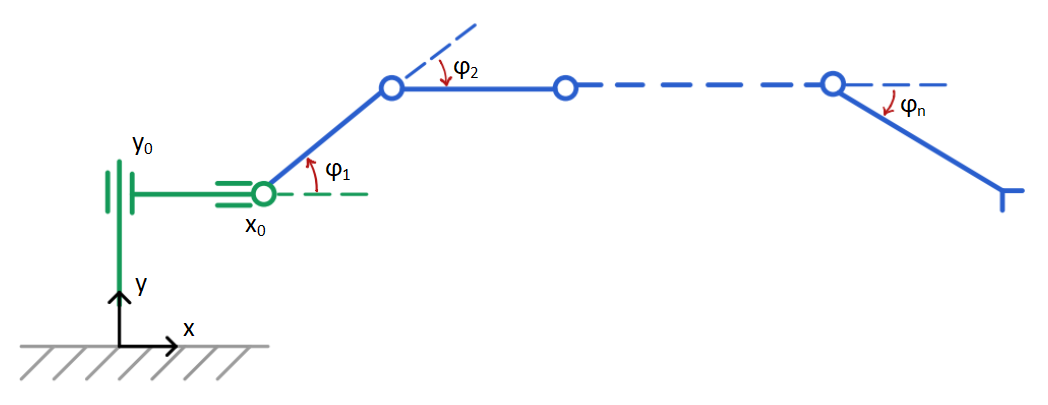
\includegraphics[width=0.9\textwidth]{figures/theory/kinematics.PNG}
    \caption{Model of snake robot with notation}
    \label{fig:kin_name}
\end{figure}


Homogeneous transformation matrices are used to express the pose (position and orientation) of the links in relation to the base frame. This means that as long as the joint angles and size of the snake robot are known, the Cartesian positions can be calculated.
The homogeneous transformation matrix for the end point of link $i$ from the base frame $b$ is given by (\ref{eq:transformationmatrix}). The base frame will stay put regardless of motion of the robot. Note also that the link length $l$ is assumed equal for all the links.

\begin{equation} \label{eq:transformationmatrix}
    \textbf{T}_{b i} = \textbf{D}_x(x_0) \textbf{D}_y(y_0) \sum_{k=1}^{i} \textbf{R}_z(\phi_k) \textbf{D}_x(l)
\end{equation}
\\
The translation and rotation matrices are given by

\begin{equation}\label{eq:trans_rot}
    \begin{split}
        \textbf{D}_x(x)& = 
        \begin{bmatrix}
            1 & 0 & x \\
            0 & 1 & 0 \\
            0 & 0 & 1
        \end{bmatrix}, \ \
        \textbf{D}_y(y) =
        \begin{bmatrix}
            1 & 0 & 0 \\
            0 & 1 & y \\
            0 & 0 & 1
        \end{bmatrix}, \ \
        \\&
        \\&\textbf{R}_z(\phi) =
        \begin{bmatrix}
            \cos{\phi} & -\sin{\phi} & 0 \\
            \sin{\phi} &  \cos{\phi} & 0 \\
            0          &  0          & 1
        \end{bmatrix}.
    \end{split}
\end{equation}
\\
The transformation matrix from the reference frame to the center of link $i$ can be found in the same manner. The only difference is that the very last translational matrix has to take the argument $l/2$ instead of $l$. This is useful to keep in mind as it be used in Section \ref{sec:dyn} for the derivation of the kinetic energy of the links.

As mentioned earlier, the transformation matrix $\textbf{T}_{b i}$ can be used to find the absolute orientation and position of the tip of link $i$ in the base frame.
The resulting matrix can be written on the form

\begin{equation}
    \textbf{T}_{b i} =
    \NORMAL{
    \begin{bmatrix}
        \textbf{R}_{b i}(\phi_{i,abs}) & \textbf{t}_{r i}^r \\
        \textbf{0}^T & 1
    \end{bmatrix} }.
\end{equation}
\\
The position is directly extracted from $\textbf{t}_{r i}^r = [x_i y_i]^T$. The orientation $\phi_{i,abs}$ is found by comparing $\textbf{R}_{b i}$ to $\textbf{R}_z$ and solving for $\phi_{i,abs}$.

Alternatively, one can directly compute the position of the center of a link $i$ from the expressions below

\begin{equation} \label{eq:pos}
    \begin{split}
        x_i &= x_0 + \sum_{k=1}^{i} l \cos{(\sum_{j=1}^{k} \phi_j)} \\
        y_i &= y_0 + \sum_{k=1}^{i} l \sin{(\sum_{j=1}^{k} \phi_j)},
    \end{split}
\end{equation}
\\
where $l$ is the link length and $1\leq i\leq n$.

\subsubsection{Forward and inverse instantaneous kinematics}\label{subseq:inst_fwd}

The well known Jacobian lets us transform between Cartesian and joint velocities. It is derived by taking the partial derivative of the $x$ and $y$ position of link $1\leq i\leq n$ with respect to all generalized coordinates

\begin{equation}\label{eq:Jc1}
    \mathbf{J_i} = 
    \HUGE{
    \begin{bmatrix}
        \frac{\partial x_i}{\partial q_1} & ... & \frac{\partial x_i}{\partial q_{N-1}} & \frac{\partial x_i}{\partial q_{N}} \\
        \frac{\partial y_i}{\partial q_1} & ... & \frac{\partial y_i}{\partial q_{N-1}} & \frac{\partial y_i}{\partial q_{N}} \\
    \end{bmatrix}
    }.
\end{equation}
\\
The relationship between the Cartesian velocity $\mathbf{v}$ of the point $(x_i, y_i)$ on the robot and the joint velocities $\mathbf{\dot{q}}$ can thus be written as 

\begin{equation}
    \mathbf{v_i = J_i(q) \dot{q}} \quad \textrm{ and } \quad \mathbf{\dot{q} = J_i(q)^\dagger v_i}.
\end{equation}
\\
The first equation is formally referred to as the forward instantaneous kinematics, whereas the second one is referred to as the inverse instantaneous kinematics.
$\mathbf{J(q)^\dagger}$ is the pseudo inverse of the Jacobian, which has to be used as a result of the Jacobian being non-square.

%------------------------------------------------------------------------------------------------

\subsection{Constrained kinematics}\label{seq:constr_kin}

%\hl{Virtual closed kinematic chain}\\
For the case in which the robot is in contact with the environment, the motion will be constrained. The obstacles found in the environment are modelled as single frictionless points. The only constraint imposed by the environment is that the robot cannot penetrate the obstacles. It can, however, both apply an arbitrary large force against them or move along them.

The model assumes that any link can be in contact with at most one obstacle at the time. To represent the mentioned constraint, the vector of generalized coordinates is expanded with $n$ further elements, where $n$ is the number of links. The updated vector $\mathbf{q}$ is now

\begin{equation} \label{eq:q2}
    \mathbf{q} = 
    \begin{bmatrix}
        \phi_1 & \phi_2 & ... & \phi_n & x_0 & y_0 & d_{c,1} & d_{c,2} & ... & d_{c,n}
    \end{bmatrix}^T,
\end{equation}
\\
where $N = 2 + 2n$ is the new number of generalized coordinates.

The newly introduced coordinates $d_{c,1}, ... , d_{c,n} \geq 0$ represent the distance to the possible contact point from the corresponding joint. For instance, the coordinate $d_{c,2}$ is the distance between the second joint and the contact point measured along the second link, as illustrated in Figure \ref{fig:3_obs_force}. Every link might not be in contact with an obstacle, but the maximum number of coordinates is introduced in the interest of keeping the vector size constant. 
Seeing as there is no actuation force directly connected to the obstacle-related coordinates, they will be referred to as virtual joints or virtual coordinates.

The position of a contact point on link $1\leq i\leq n$ in the base frame can be derived through the corresponding transformation matrix (\ref{eq:obst_tfmatrix}).

\begin{equation} \label{eq:obst_tfmatrix}
    \textbf{T}_{b ci} = \textbf{D}_x(x_0) \textbf{D}_y(y_0) \sum_{k=1}^{i-1} (\textbf{R}_z(\phi_k) \textbf{D}_x(l)) \textbf{R}_z(\phi_i) \textbf{D}_x(d_{c,1})
\end{equation}

\begin{figure}
    \centering
    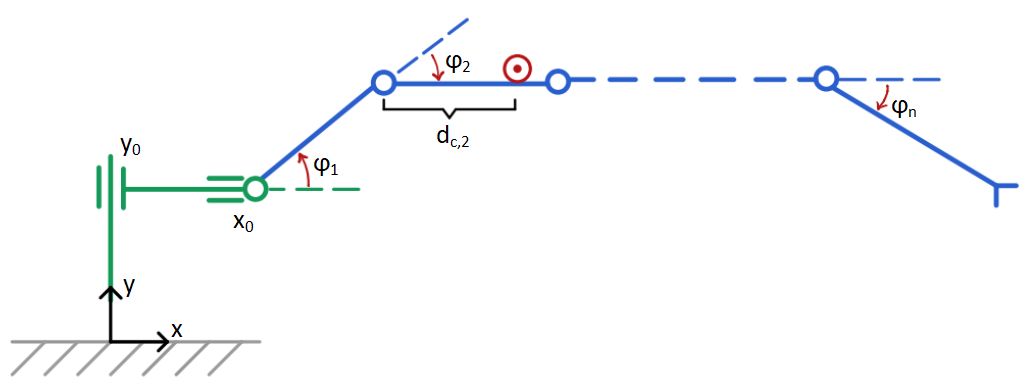
\includegraphics[width=0.9\textwidth]{figures/theory/contact_point.PNG}
    \caption{Snake robot in contact with obstacle}
    \label{fig:3_obs_force}
\end{figure}


%------------------------------------------------------------------------------------------------

\subsubsection{Constrained instantaneous kinematics}\label{subseq:constr_inst}

The Jacobian matrix related to the velocity of the contact point can be derived in the same manner as in the unconstrained case. The only difference is that the partial differentiation of the contact point $(x_c,y_c)$ is now taken with respect to the extended vector of generalized coordinates (\ref{eq:q2}). The resulting contact Jacobian for a contact point on link $1\leq i\leq n$ is thus

\begin{equation}\label{eq:Jac_constr}
    J_{c,i} = 
    \HUGE{
    \begin{bmatrix}
        \frac{\partial x_{c,i}}{\partial \phi_2} & ... & \frac{\partial x_{c,i}}{\partial q_{N-1}} & \frac{\partial x_{c,i}}{\partial q_N} \\
        \frac{\partial y_{c,i}}{\partial \phi_2} & ... & \frac{\partial y_{c,i}}{\partial q_{N-1}} & \frac{\partial y_{c,i}}{\partial q_N} \\
    \end{bmatrix}
    }.
\end{equation}
\\
This Jacobian will end up being quite sparse, seeing as the coordinate of a contact point is independent of all other contact coordinates. This is a property that can be exploited using sparse solvers if the snake robot has a large number of links.

The relationships between the Cartesian velocity of a contact point on link $1\leq i\leq n$ and the joint velocities can now be expressed as

\begin{equation}
    \mathbf{v_{c,i} = J_{c,i}(q) \dot{q}} \quad \textrm{ and } \quad \mathbf{\dot{q} = J_{c,i}(q)^\dagger v_{c,i}}.
\end{equation}



\section{Snake robot dynamics} \label{sec:dyn}

This section, similar to the last section, is taken from \cite{AtussaProsjektoppgp}. The only modifications made are the variable notations and an error fix in (\ref{eq:k_rot}).

The snake robot has $n-1$ joint actuators that all can apply torques to their corresponding joints. The dynamics describe how the robot moves in response to these actuator forces. For simplicity, it is assumed that the actuators do not have dynamics of their own and, hence, arbitrary torques can be commanded at the joints of the robot \cite{murray2017mathematical}.

The dynamics of the snake robot will be expressed using the joint space equations of motion formulation

\begin{equation}
    \mathbf{M(q)\ddot{q} + C(q, \dot{q}) + g(q)} = \boldsymbol{\tau}.
\end{equation}
\\
Because the movement is restricted to the 2D plane, the gravitational term $\mathbf{g(q)}$ can be neglected and the equations of motion can be rewritten to

\begin{equation}\label{eq:eom}
    \mathbf{M(q)\ddot{q} + C(q, \dot{q})} = \boldsymbol{\tau},
\end{equation}
\\
where $\mathbf{M(q)}$ and $\mathbf{C(q,\dot{q})}$ is the mass matrix and Coriolis matrix respectively.
$\boldsymbol{\tau}$ is the vector of generalized torques corresponding to the generalized coordinates (\ref{eq:q}). Furthermore, the elements corresponding to the virtual coordinates will be zero at all times.

Solving (\ref{eq:eom}) with respect to $\mathbf{\ddot{q}}$ yields

\begin{equation}\label{eq:eom_qdd}
    \mathbf{\ddot{q}} = \mathbf{M^{-1}(q)}( \boldsymbol{\tau} - \mathbf{C(q, \dot{q})}).
\end{equation}
\\
Several methods exist for finding the equations of motion for a robot. The Euler-Lagrange method \cite{lynch2017modern}, which  is chosen here, is based on the difference in kinetic energy ($K$) and potential energy ($P$) of the system, also known as the Lagrangian

\begin{equation}
    L = K - P.
\end{equation}
\\
The equations of motion can now be expressed as a second order partial differential equation

\begin{equation} \label{eq:Lagrange}
    \frac{d}{d t} \frac{\partial L}{\partial \mathbf{\dot{q}}} - \frac{\partial L}{\partial \mathbf{q}} = \boldsymbol{\tau}.
\end{equation}
\\
Again, simplifications can be made from the restricted movement in the world and thus the potential energy $P$ can be neglected. The Lagrangian is therefore simply equal to the kinetic energy, which is the sum of the kinetic energy for every link \cite{rezapour2014path}. Furthermore, the kinetic energy for one link $i$ is divided into two parts, $K_{translational}$ and $K_{rotational}$.
The kinetic energy can now be express as

\begin{equation}\label{eq:kinen}
    K = \sum_{i=1}^{n} (K_{translational,i} + K_{rotational,i}),
\end{equation}
\\
where the translational and rotational kinetic energy is given in (\ref{eq:k_trans}) and (\ref{eq:k_rot}) respectively.

\begin{equation} \label{eq:k_trans}
    K_{translational,i} = \frac{1}{2} m (\dot{x}_i^2 + \dot{y}_i^2)
\end{equation}
\\
Here $m$ is the link mass, and $(\dot{x}_i, \dot{y}_i)$ make out the velocity of the center of the link found by differentiating (\ref{eq:pos}) with respect to time. 

\begin{equation} \label{eq:k_rot}
    K_{rotational,i} = \frac{1}{2}I\dot{\theta}_i^2
\end{equation}
\\
$\dot{\theta}_{i}$ is the rotational velocity of link $i$ with respect to the base frame. Furthermore, every link has the same moment of inertia, namely $I = (1/12)ml^2$. This is the moment of inertia of a rod, corresponding to the moment of inertia of a cylinder with zero radius \cite{lynch2017modern}.


%------------------------------------------------------------------------------------------------

%\subsection{Constrained dynamics}\label{subseq:constr_dyn}




%\section{The obstacle triplet model} \label{sec:obst_triplet_model}

\section{Snake robot constraint formulation}\label{seq:constraints}

Figure \ref{} illustrates the used model of the snake robot and its environment. \hl{A figure and some more explanation of the figure.}

When looking at this model, it is evident that the snake robot will experience constraints if it tries to move its links in the directions of the obstacles. One way of expressing this constraint is limiting the velocity of the link in contact. The position of contact on link $i$ was in \ref{subseq:constr_inst} denoted as $(x_{c,i}, y_{c,i})$. Following, the corresponding velocity $\mathbf{v}_{c,i}$ can be written $(\dot{x}_{c,i}, \dot{y}_{c,i})$.

It is not the general velocity of this point that is constrained, but rather the velocity normal to the link. This follows from the assumption of the contact being a point contact. The normal velocity can be found with the use of the angle $\theta_i$ of link $i$ with respect to the base frame. From basic trigonometric laws, the normal velocity is found to be

\begin{equation}\label{eq:norm_vel}
    v_{nc,i} = -sin(\theta_i) \dot{x}_{c,i} + cos(\theta_i) \dot{y}_{c,i}.
\end{equation}
\\
Since there can only be one contact per link and the contact can only take place at one side of the link at the time, the link can still move away from the obstacle with a velocity normal to the link. Holden et al. \cite{holden2014optimal} introduce a variable $\gamma_i$ that holds information about which side of the link the obstacle is positioned. The variable can take the values ${-1, 0, 1}$, where $\gamma_i=1$ for obstacles to the right of the link and vice versa. For links not in contact with any obstacles $\gamma_i=0$.

The allowed normal direction of movement for link $i$ can now be expressed as

\begin{equation}\label{eq:norm_vel2}
    \gamma_i v_{nc,i} \geq 0.
\end{equation}
\\
It might be desired to stay in touch with the obstacle for propulsion purposes. Because of this, it is reasonable to simplify the constraint equation to not let the contact point on the link move in any normal direction to the link at that point. The constraint can thus now be expressed as

\begin{equation}\label{eq:norm_vel3}
    \gamma_i v_{nc,i} = \gamma_i(-sin(\theta_i) \dot{x}_{c,i} + cos(\theta_i) \dot{y}_{c,i}) = 0
\end{equation}
\\
Moreover, the side of the contact is insignificant if the velocity is limited in both directions. (\ref{eq:norm_vel3}) is further simplified to

\begin{equation}\label{eq:norm_vel4}
    v_{nc,i} = -sin(\theta_i) \dot{x}_{c,i} + cos(\theta_i) \dot{y}_{c,i} = 0.
\end{equation}
\\

\chapter{Dynamic hybrid position/force control for snake robots}

\section{Hybrid position/force controllers}

The goal of the snake robot is to push against obstacles in a fashion that yields forward propulsion along a path. Consequently, the robot will have to curve itself along the path whilst applying a force to the obstacles considered advantageous. The behavior of the robot has to comprise with the constraints arising from the contact, which further motivates the use of hybrid position/force control (HPFC).

HPFC is not a control method per se, but rather a method for determining when and in which directions force or motion control should be applied. It is desired to control motion along the unconstrained motion directions and force along the constrained motion directions. Different approaches to this problem exist. One is the use of selection matrices, introduced by Raibert and Craig et al. \cite{raibert1981hybrid}. The disadvantage of this approach is that the directions in which force and motion should be controlled has to be recalculated for every step, and is no simple procedure. In another approach, introduced by West and Asada \cite{west1985method}, two projection matrices are used as filters in joint space to automatically select between position- and force controlled vectors. There is however a disadvantage to this method as well, which is that the dynamics of the robot are ignored. A thoroughly studied method called dynamic HPFC, developed by Yoshikawa \cite{yoshikawa1987dynamic}, is therefore presented and adapted to the snake robot.

The theory on traditional HPFC up until the part \textit{Passive joints}, as well as this intro, is a modified part of the earlier project work of the author \cite{AtussaProsjektoppgp}. The rest of the chapter is focused on dynamic HPFC and the advantages and challenges that comes with adapting it to a snake robot model.

\subsection{Traditional HPFC} \label{subseq:HPFC}

Like mentioned above, velocity and force can be controlled in the directions in which they are not constrained. The end effector space of a robot can be divided into two orthogonal domains, a position domain and a force domain. These domains are complementary to the directions of the corresponding constraints at the end effector. It is logical to conclude that if there is contact with the environment, motion cannot be controlled freely. On the other hand, if there is no contact, there is no direction in which the robot can apply a force. Ergo, the force and motion control directions do not overlap and the domains are orthogonal. This means that position and force can be controlled independently and arbitrarily in these domains.

The following relationships are known from \ref{seq:constr_kin} and \ref{subseq:constr_dyn}. 

\begin{equation}
	\mathbf{v = J \dot{q}} \textrm{,} \quad  \  \boldsymbol{\tau} \mathbf{= J}^T \mathbf{f}
\end{equation}
\\
An important observation is that constraints due to contact with the environment are constraints due to a closed kinematic chain. In general, this is something that occurs when at least \textit{two} points of the robot are in contact with the environment. For the snake robot this might not always be the case. It is however possible to define a virtual closed kinematic chain where the robot is connected to the base with the virtual joint variables $x_0$, $y_0$ and $\phi_0$.
A separate Jacobian is calculated for each closed kinematic chain, as explained in \ref{subseq:constr_inst}.
%These Jacobians are denoted $\mathbf{J_{ci}}$, where $i = 1, .., k$ is the number of independent closed kinematic chains.
%Since the motion is constrained at a contact point, the relationships

Relationship (\ref{eq:constr_dyns}) comes from the motion being constrained at a contact point.

\begin{equation} \label{eq:constr_dyns}
    \mathbf{\dot{v}_{ci} = J_{ci} \dot{q} = 0}
\end{equation}
\\
The solution to (\ref{eq:constr_dyns}) can be proven to be

\begin{equation}
    \mathbf{\dot{q} = (I - J_{ci}^+ J_{ci}) y},
\end{equation}
\\
where $\mathbf{y}$ can be an arbitrary vector, as it will yield zero end effector motion. Furthermore, since the matrix $\mathbf{J_{ci}}$ might be non square, the pseudo inverse $\mathbf{J_{ci}^+}$ is used.
For a closed kinematic chain, the work done at the end of the chain must also be zero. Therefore, the sum of the work done by each of the joints must be zero:

\begin{equation} \label{eq:zero_joint_work}
    \boldsymbol{\tau^T} \mathbf{\dot{q}} = \boldsymbol{\tau^T} \mathbf{(I - J_{ci}^+ J_{ci}) y = 0}.
\end{equation}
\\
(\ref{eq:zero_joint_work}) has the general solution

\begin{equation}
   \boldsymbol{\tau}  \mathbf{= (J_{ci}^+ J_{ci})^T z},
\end{equation}
\\
where $\mathbf{z}$ can be an arbitrary vector.

The allowable motion is now characterized by $\mathbf{[I - J_{ci}^+ J_{ci}]}$ and the allowable forces by $\mathbf{[J_{ci}^+ J_{ci}]^T}$. These matrices are orthogonal projectors in joint space onto the allowable position and force variations respectively. A further explanation of this result is given in Chapter 5 of \cite{west1985method}. The projectors will be abbreviated to

\begin{equation}\label{eq:proj_mtrices}
    \prescript{}{j}{\mathbf{P}}_{ap} = \mathbf{[I - J_{ci}^+ J_{ci}]} \ \ \quad \textrm{and} \quad
    \prescript{}{j}{\mathbf{P}}_{af} = \mathbf{[J_{ci}^+ J_{ci}]^T = [I - (\prescript{j}{ap}{P})^T]}.
\end{equation}
\\
The subscript $j$ denotes joint space, and $ap$ and $af$ stand for allowable positions and allowable forces respectively. It can be observed that these projection matrices project onto the nullspace of the respective constraint directions. This can further be related to the concept of task priority, in which tasks with lower priority are performed in the null-space of higher priority tasks \cite{chiaverini2008kinematically}. An important observation is that the mapping onto the allowable force and position spaces are in this method purely determined by the kinematics of the robot.

\subsubsection{Multiple constraints}\label{subseq:mult_contacts}

If there are several contact points, projection matrices are calculated for each constraint, and the final projection matrices are found by taking the union and intersect of the different $\prescript{}{j}{\mathbf{P}}_{af}$ and $\prescript{}{j}{\mathbf{P}}_{ap}$ respectively.

\subsubsection{Passive joints}

The presence of passive joints in the robot imposes another constraint on the allowable forces. This is because the force in a passive joint is uncontrollable. \cite{west1985method} presents two methods of including this constraint. One of which is using a diagonal matrix $\mathbf{A}$ that denotes which joints are passive and which are active. A 1 on the diagonal indicates an active joint whereas a 0 indicates a passive joint. This matrix has to be manually initialized before controlling the robot. It can then be combined with the allowable force projection by taking the intersect of the space spanned by $\mathbf{A}$ and $\prescript{}{j}{\mathbf{P}}_{af}$.

\subsubsection{Task analysis}

An end effector task may consist of both a movement and force application onto a surface. The projectors $\prescript{}{j}{\mathbf{P}}_{ap}$ and $\prescript{}{j}{\mathbf{P}}_{af}$ make sure the force and movement are performed in the allowable force and movement directions. A specific task may however not be possible to perform within the restrictions of these spaces.

\textit{Essential position variables} are defined as the directions om movement of the end effector which must be controlled in order to perform the task correctly. At the same time, \textit{arbitrary position variables} are those directions of movement which do not have to be controlled precisely. The terms \textit{essential force variables} and \textit{arbitrary force variables} follow the same logic, just for the force directions. According to \cite{west1985method}, the total number of essential variables, position plus force, is equal to the minimum number of controllable actuators in the manipulator necessary for performing the task.

The essential position and force direction can be described by the column vectors (\ref{eq:hpfc_ep}) and (\ref{eq:hpfc_ef}) respectively.

\begin{equation}\label{eq:hpfc_ep}
    \mathbf{E}_p =
    \begin{bmatrix}
        \mathbf{e}_{p1} & ... & \mathbf{e}_{p\alpha}
    \end{bmatrix}^T
\end{equation}

\begin{equation}\label{eq:hpfc_ef}
    \mathbf{E}_f =
    \begin{bmatrix}
        \mathbf{e}_{f1} & ... & \mathbf{e}_{f\beta}
    \end{bmatrix}^T
\end{equation}
\\
Each column vector describes one direction. Following, the number of essential position directions is $\alpha$ and the number of essential force directions is $\beta$. The orthogonal projections onto the essential position and force spaces are given by (\ref{eq:hpfc_wep}) and (\ref{eq:hpfc_wef}) respectively.

\begin{equation}\label{eq:hpfc_wep}
    \prescript{}{w}{\mathbf{P}}_{ep} = \mathbf{E}_p(\mathbf{E}_p^T \mathbf{E}_p)^{-1} \mathbf{E}_p^T
\end{equation}

\begin{equation}\label{eq:hpfc_wef}
    \prescript{}{w}{\mathbf{P}}_{ef} = \mathbf{E}_f(\mathbf{E}_f^T \mathbf{E}_f)^{-1} \mathbf{E}_f^T
\end{equation}
\\
The inverse in the two equations above is, probably by mistake, not included in \cite{west1985method}. The $w$ denotes that the projectors are defined in work space coordinates. In order to combine these projectors with the allowable position and force projectors, it is desirable to define them in the joint space coordinate system. The precondition for this to be possible for the essential position space is that the number of joints linking the base of the manipulator to the end effector is greater than or equal to three (given the two dimensional case). For the essential force space, the number of \textit{active} joints has to be greater than or equal to three. The joint space projectors can then be found by

\begin{equation}\label{eq:hpfc_jep}
    \prescript{}{j}{\mathbf{P}}_{ep} = \mathbf{J}_t^+ \prescript{}{w}{\mathbf{P}}_{ep} \mathbf{J}_t
\end{equation}

\begin{equation}\label{eq:hpfc_jeF}
    \prescript{}{j}{\mathbf{P}}_{ef} = \mathbf{J}_c^+ \prescript{}{w}{\mathbf{P}}_{ef} (\mathbf{J}_c^T)^+
\end{equation}
\\
The Jacobian $\mathbf{J}_t$ relates the task specific coordinates to the joint space. Section \ref{subsec:DHPFC} explains how this Jacobian can be found for the snake robot case.

Eventually, the projections in joint space that project onto the allowable motion and force spaces \textit{and} result in the desired motion and force necessary to perform the task are given by (\ref{eq:hpfc_fp}) and (\ref{eq:hpfc_ff}) respectively.

\begin{equation}\label{eq:hpfc_fp}
    \prescript{}{j}{\mathbf{F}}_{p} = \prescript{}{j}{\mathbf{P}}_{ap} (\prescript{}{j}{\mathbf{P}}_{ep} \prescript{}{j}{\mathbf{P}}_{ap})^+ \prescript{}{j}{\mathbf{P}}_{ep}
\end{equation}

\begin{equation}\label{eq:hpfc_ff}
    \prescript{}{j}{\mathbf{F}}_{f} = \prescript{}{j}{\mathbf{P}}_{af} (\prescript{}{j}{\mathbf{P}}_{ef} \prescript{}{j}{\mathbf{P}}_{af})^+ \prescript{}{j}{\mathbf{P}}_{ef}
\end{equation}

\subsection{Dynamic HPFC} \label{subsec:DHPFC}

The solution of West and Asada \cite{west1985method} does not take the manipulator dynamics into account. Nevertheless, in a real system, the dynamics play a significant role in the resulting behavior of the robot. For this reason, Yoshikawa \cite{yoshikawa1987dynamic} designed the dynamic hybrid control method which incorporates the constraints into the manipulator dynamics. More specifically, the solution of \cite{west1985method} filters the commanded joint torques and velocities to conform to the constraints and the essential variable space. This is explained in more detail in \ref{subseq:HPFC}. The essence of the solution of \cite{yoshikawa1987dynamic} however, is that the robot dynamics and constraint equations are combined before the commanded torques and angles are calculated. 

This section aims at describing the improved method, and the content is based the paper of \cite{yoshikawa1987dynamic}. The symbolic conventions used are for simplicity the same as in the paper. The next section will explain further how the theory and these symbols apply to the snake robot case and the snake robot specific theory presented earlier in this chapter (\ref{sec:kin}-\ref{seq:constraints}).

It is worth noting that the solution of Yoshikawa is designed for a robot manipulator with a static base where the only constraint present is targeted at the manipulator end effector. For this reason, special effort has been put into finding a suitable formulation of the snake robot constraints. Additionally, the difference between the coordinate spaces introduced in the paper are easy to confuse and special attention has been directed at thoroughly defining these spaces for the snake robot so that the following calculations can be both as clear and logical as possible.

\subsubsection{Description of variables}

A brief overview of the most significant new variables used in this section is provided below.
The most general variables correspond to the ones presented in \ref{sec:kin}.

\begin{itemize}
    \item $\mathbf{r_t}$: task coordinates related to the contact point (task) coordinate system
    \item $\mathbf{r_c}$: constraint coordinates related to the fixed obstacle coordinate system
    \item $\mathbf{E}_F$: axes of constraints on the force in the task frame
    \item $\mathbf{E}_P$: axes of constraints on the position in the task frame
    \item $\mathbf{J}_t$: Jacobian relating the joint coordinates $\dot{\mathbf{q}}$ to the task coordinates $\dot{\mathbf{r}}_t$
    \item $\boldsymbol{\tau}_c$: control torque
    \item $\boldsymbol{\tau}_F$: torque from the desired force
    \item $\boldsymbol{\tau}_P$: torque from the desired position
\end{itemize}

The task and obstacle frames $\mathbf{r_t}$ and $\mathbf{r_c}$ are visualized in Figure \ref{fig:rt-rc}. The values for both $r_{t,i} = [x_{t,i}, y_{t,i}, \theta_{t,i}]$ and $r_{c,i} = [x_{c,i}, y_{c,i}, \theta_{c,i}]$ are defined with respect to the base frame.

\begin{figure}
    \centering
    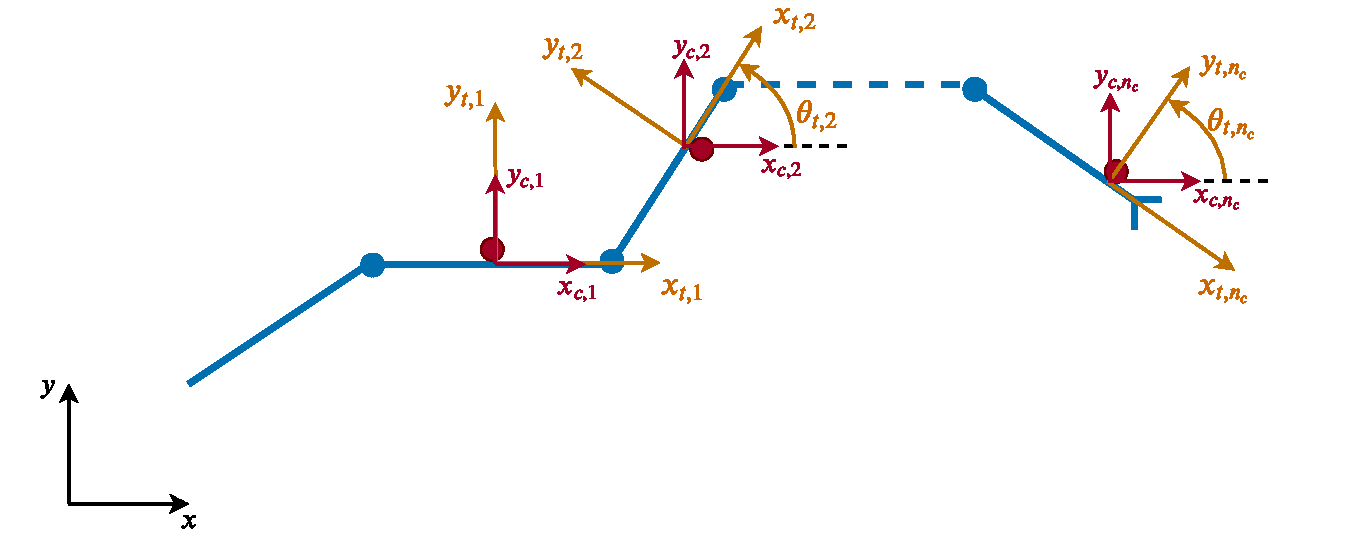
\includegraphics[width=\textwidth]{figures/theory/rt-rc.pdf}
    \caption{Model of snake robot and obstacles illustrating the task and contact frames}
    \label{fig:rt-rc}
\end{figure}


\subsubsection{Description of constraints}

In order to take the dynamics into account, the constraints are directly included into the dynamic equations of motion of the robot. This is done by expressing the constraints as a set of hypersurfaces that the robot can not physically pass. It should be noted that the focus here is on manipulator end-effector constraints and not general constraints which should be used in the snake robot case. The constraint hypersurfaces are also expressed in the end-effector coordinates. Another important aspect of the paper is that it only addresses bilateral hypersurfaces (and not unilateral surfaces), meaning that the effector is prohibited from leaving the surface in any direction.

It is assumed that a given constraint can be expressed by a set of $m$ hypersurfaces

\begin{equation}\label{eq:hpfc:hypersurface}
    p_i(\mathbf{r}_t) = 0, \quad i = 1, 2, ..., m,
\end{equation}
\\
where $\mathbf{r}$ is the end effector position in a fixed reference frame. Differentiating (\ref{eq:hpfc:hypersurface}) with respect to time yields

\begin{equation}\label{eq:hpfc:derhypsurf}
    \mathbf{E}_F \mathbf{\dot{r}}_t = 0,
\end{equation}
\\
where the vectors of $\mathbf{E}_F$ are the unit normal vectors to the hypersurfaces in (\ref{eq:hpfc:hypersurface}).

By comparing the expression (\ref{eq:norm_vel5}) of the constraint on link $i$ found in \ref{seq:constraints} to (\ref{eq:hpfc:derhypsurf}), it is possible to extract the matrix $\mathbf{E}_{F,i}$ and a logical choice of $\mathbf{r}_{t,i}$ and $\mathbf{\dot{r}}_{t,i}$ presents itself.
Specifically, if one chooses

\begin{equation}
    \mathbf{r}_{t,i} =
    \begin{bmatrix}
        x_{t,i} & y_{t,i} & \theta_{t,i}
    \end{bmatrix}^T \in \mathcal{R}^3,
\end{equation}
\\
then $\mathbf{\dot{r}}_{t,i} = [\dot{x}_{t,i}, \dot{y}_{t,i}, \dot{\theta}_{t,i}]^T \in \mathcal{R}^3$ and the matrix $\mathbf{E}_{F,i}$ can by comparison be found as

\begin{equation}
    \mathbf{E}_{F,i} =
    \begin{bmatrix}
        0 & 1 & 0
    \end{bmatrix} \in \mathcal{R}^3.
\end{equation}
\\
The subscript $i$ will now be used as the constraint number, where $n_c$ is the number of constraints/contact points.
The angle of the link at the contact point $\theta_{t,i}$ with respect to the base frame is the same as the angle $\theta$ of the link in contact with respect to the base frame (see Figure \ref{fig:rt-rc}). It can by inspection be seen that $\mathbf{E}_{F,i}$ fulfills the criteria of being of unit size.

%These formulations do not supply an explicit expression of the corresponding constraint hypersurface. It is however not a necessity for the further computations. On the other hand it could be valuable to have the expressions for the hypersurfaces for analysis purposes.

The coordinate space $\mathbf{r}_t$ should be able to aid in expressing all the constraints present on the snake robot. Therefore, it is chosen as 

\begin{equation}
    \mathbf{r}_t = 
    \begin{bmatrix}
        \mathbf{r}_{t,1}^T & \mathbf{r}_{t,2}^T & \dots &\mathbf{r}_{t,n_c}^T
    \end{bmatrix}^T \in \mathcal{R}^{3 n_c}.
\end{equation}
\\
The same goes for $\dot{\mathbf{r}}_t$. Furthermore, the matrix $\mathbf{E}_{F}$ describing the unit normal vectors to all the hypersurfaces can now be written as

\begin{equation}
    \mathbf{E}_F = 
    \begin{bmatrix}
        \mathbf{E}_{F,1} & \mathbf{0}_{1\times3} & \dots & \mathbf{0}_{1\times3} \\
        \mathbf{0}_{1\times3} & \ddots & & \vdots \\
        \vdots & & \ddots & \mathbf{0}_{1\times3} \\
        \mathbf{0}_{1\times3} & \dots & \mathbf{0}_{1\times3} & \mathbf{E}_{F,n_c} \\
    \end{bmatrix} \in \mathcal{R}^{n_c \times 3 n_c}
\end{equation}
\\

Differentiating (\ref{eq:hpfc:derhypsurf}) further gives

\begin{equation}\label{eq:dhpfc_arf}
    \mathbf{E}_F \mathbf{\ddot{r}}_t + \mathbf{a}_{r F} = 0, \quad \mathbf{a}_{r F} = \mathbf{\dot{E}}_F\mathbf{\dot{r}}
\end{equation}
\\
For the snake robot case $\mathbf{a}_{r F} \in \mathcal{R}^{n_c}$.

Furthermore, $\mathbf{E}_P$ is chosen so that all the vectors in the relation

\begin{equation}\label{eq:dhpfc_E}
    \mathbf{E} =
    \begin{bmatrix}
    \mathbf{E}_P \\ \mathbf{E}_F
    \end{bmatrix}
\end{equation}
\\
are mutually independent unit vectors. The matrix $\mathbf{E}_F$ represents the coordinate axes normal to the constraint surfaces, and $\mathbf{E}_P$ represents the coordinate axes complementing $\mathbf{E}_F$. Another way to display this is seeing $\mathbf{E}_F$ and $\mathbf{E}_P$ as the axes for force and position constrained directions respectively.

From the equations

\begin{equation}
    \mathbf{E\dot{r}} =
    \begin{bmatrix}
        \mathbf{E}_P \mathbf{\dot{r}}_t\\
        0
    \end{bmatrix}
    \quad \text{and} \quad
    \mathbf{E\ddot{r}}_t =
    \begin{bmatrix}
        \mathbf{E}_P \mathbf{\ddot{r}}_t \\
        -\mathbf{a}_{r F}
    \end{bmatrix}
\end{equation}
\\
it can be seen that the velocity to the constraint surface is zero, which is natural seeing as the end-effector should be physically unable to move through the surface.

For the snake robot, a simple choice of $\mathbf{E}_{P,i}$ with unit vectors complementing $\mathbf{E}_{F,i}$ is by inspection found to be

\begin{equation}\label{eq:dhpfc_EPi}
    \mathbf{E}_{P,i} = 
    \begin{bmatrix}
        1 & 0 & 0 \\
        0 & 0 & 1
    \end{bmatrix} \in \mathcal{R}^{2\times 3}.
\end{equation}
\\
This is a very logical choice, seeing as the snake robot link in contact is allowed to rotate about the obstacle and move along the obstacle.
Again, $\mathbf{E}_{P,i}$ corresponds to the $i$'th constraint. Combining all $\mathbf{E}_{P,i}$ gives 

\begin{equation}
    \mathbf{E}_P = 
    \begin{bmatrix}
        \mathbf{E}_{P,1} & \mathbf{0}_{2\times3} & \dots & \mathbf{0}_{2\times3} \\
        \mathbf{0}_{2\times3} & \ddots & & \vdots \\
        \vdots & & \ddots & \mathbf{0}_{2\times3} \\
        \mathbf{0}_{2\times3} & \dots & \mathbf{0}_{2\times3} & \mathbf{E}_{P,n_c} \\
    \end{bmatrix} \in \mathcal{R}^{2 n_c \times 3 n_c}
\end{equation}
\\
and $\mathbf{E} \in \mathcal{R}^{3 n_c \times 3 n_c}$.

%%%%%%%%%%%%%%%%%%%%%%%%%%%%%%%%%%%%%%%%%%%%%%%%%%%%%%%%%%%%%%%%%%%%%%%%%%%%%%%%%%%%%%%%%%%%%
%%%%%%%%%%%%%%%%%%%%%%%%%%%%%%%%%%%%%%%%%%%%%%%%%%%%%%%%%%%%%%%%%%%%%%%%%%%%%%%%%%%%%%%%%%%%%
%%%%%%%%%%%%%%%%%%%%%%%%%%%%%%%%%%%%%%%%%%%%%%%%%%%%%%%%%%%%%%%%%%%%%%%%%%%%%%%%%%%%%%%%%%%%%

\subsubsection{Kinematics and dynamics}

In \cite{yoshikawa1987dynamic}, the relation between the joint variable vector $\mathbf{q}$ and the end effector position $\mathbf{r}_t$ is expressed as

\begin{equation}\label{eq:hpfc:rq}
    \mathbf{r}_t = \mathbf{c(q)}.
\end{equation}
\\
The following equations are generated by differentiating \ref{eq:hpfc:rq}.

\begin{equation}
    \mathbf{\dot{r}}_t = \mathbf{J}_t \mathbf{\dot{q}}, \quad \mathbf{J}_t = \frac{\partial \mathbf{c(q)}}{\partial \mathbf{q}^T}
\end{equation}

\begin{equation}\label{eq:dhpfc_aq}
    \mathbf{\ddot{r}}_t = \mathbf{J}_t \mathbf{\ddot{q}} + \mathbf{a}_q, \quad \mathbf{a}_q = \mathbf{\dot{J}}_t \mathbf{\dot{q}}   
\end{equation}
\\
For the snake robot case, the matrix $\mathbf{J}_t$ is the Jacobians of all the contacts.

\begin{equation}
    \mathbf{J}_t = 
    \begin{bmatrix}
        \mathbf{J}_{t,1} \\ \mathbf{J}_{t,2} \\ \vdots \\ \mathbf{J}_{t,n_c}
    \end{bmatrix} \in \mathcal{R}^{3 n_c \times N}
\end{equation}
\\
The Jacobian is also explained in the mentioned section. The Jacobian $\mathbf{J}_{t,i} \in \mathcal{R}^{3\times N}$ for a single contact point with respect to the contact point task variable vector $\mathbf{r}_{t,i}$ is found as 

\begin{equation}
    \mathbf{J}_{t,i} =
    \HUGE{
    \begin{bmatrix}
        \frac{\partial x_{t,i}}{\partial q_1} & \dots & \frac{\partial x_{t,i}}{\partial q_N} \\
        \frac{\partial y_{t,i}}{\partial q_1} & \dots & \frac{\partial y_{t,i}}{\partial q_N} \\
        \frac{\partial \theta_{t,i}}{\partial q_1} & \dots & \frac{\partial \theta_{t,i}}{\partial q_N}
    \end{bmatrix}
    }.
\end{equation}
\\
Furthermore, $\mathbf{a}_q \in \mathcal{R}^{n_c}$.


%%%%%%%%%%%%%%%%%%%%%%%%%%%%%%%%%%%%%%%%%%%%%%%%%%%%%%%%%%%%%%%%%%%%%%%%%%%%%%%%%%%%%%%%%%%%%
%%%%%%%%%%%%%%%%%%%%%%%%%%%%%%%%%%%%%%%%%%%%%%%%%%%%%%%%%%%%%%%%%%%%%%%%%%%%%%%%%%%%%%%%%%%%%
%%%%%%%%%%%%%%%%%%%%%%%%%%%%%%%%%%%%%%%%%%%%%%%%%%%%%%%%%%%%%%%%%%%%%%%%%%%%%%%%%%%%%%%%%%%%%

\subsubsection{Calculation of the joint driving force}

The torque resulting from the contact force is found by

\begin{equation}
    \boldsymbol{\tau}_F = \mathbf{J}_t^T \mathbf{E}_F^T \mathbf{f}_F.
\end{equation}
\\
The total torque $\boldsymbol{\tau}$ applied to the robot will be the difference between the motor torque $\boldsymbol{\tau}_c$ and the constraint torque $\boldsymbol{\tau}_F$.

\begin{equation}\label{eq:tau_dhpfc1}
    \boldsymbol{\tau} = \boldsymbol{\tau}_c - \boldsymbol{\tau}_F
\end{equation}
\\

Combining the torque in (\ref{eq:tau_dhpfc1}) with the equations of motion given in (\ref{eq:eom}) gives

\begin{equation}\label{eq:dhpfc_stuff1}
    \mathbf{M(q) \ddot{q}} + \mathbf{J}_t^T \mathbf{E}^T_F \mathbf{f}_F = \boldsymbol{\tau}_c - \mathbf{C(q, \dot{q})}
\end{equation}
\\
and
\begin{equation}\label{eq:dhpfc_stuff2}
    \mathbf{E}_F \mathbf{J}_t\mathbf{\ddot{q}} = - \mathbf{E}_F \mathbf{a}_q - \mathbf{a}_{rF}.
\end{equation}
\\
Lastly, it can be shown that combining (\ref{eq:dhpfc_stuff1}) and (\ref{eq:dhpfc_stuff2}) yields the expressions

\begin{equation}
    \mathbf{\ddot{q}} = \mathbf{M}^{-1}(\mathbf{b}_1 + (\mathbf{E}_F \mathbf{J}_t)^T \mathbf{K} (\mathbf{b}_2 - \mathbf{E}_F \mathbf{J}_t \mathbf{M}^{-1} \mathbf{b}_1)),
\end{equation}

\begin{equation}
    \mathbf{f}_F = -\mathbf{K} (\mathbf{b}_2 - \mathbf{E}_F \mathbf{J}_t \mathbf{M}^{-1} \mathbf{b}_1).
\end{equation}
\\
$\mathbf{K}$, $\mathbf{b}_1$ and $\mathbf{b}_2$ are given by

\begin{equation}
    \begin{split}
        \mathbf{K} &= (\mathbf{E}_F \mathbf{J}_t \mathbf{M}^{-1} \mathbf{J}_t^T \mathbf{E}^T_F)^{-1}\\
        \mathbf{b}_1 &= \boldsymbol{\tau}_c - \mathbf{C(q, \dot{q})}\\
        \mathbf{b}_2 &= - \mathbf{E}_F \mathbf{a}_q - \mathbf{a}_{rF}.
    \end{split}
\end{equation}
\\
Eventually, it is possible to calculate the joint control torque. It consists of a component based on the desired movement $\mathbf{\ddot{r}}_{t,d}$ in the contact point frame and a component based on the desired force $\mathbf{f}_{Fd}$ applied to the constraint surfaces. The direction of the desired force should correspond to which side of the snake robot the obstacle is. This can either be implemented into the higher level controller requesting these forces, or one could introduce a vector $\boldsymbol{\gamma}$ like in \ref{seq:constraints}. This vector consists of positive and negative ones corresponding to the different obstacle placements. When multiplied with $\mathbf{f}_{Fd}$ it will simply negate the forces that should be applied to obstacles on the right side of the snake robot.

\begin{equation}\label{eq:dhpfc_tau_c}
    \boldsymbol{\tau}_c = \boldsymbol{\tau}_P + \boldsymbol{\tau}_F
\end{equation}
\\
The torque $\boldsymbol{\tau}_P$ is found by solving the equations of motion given in (\ref{eq:eom}) based on the desired values of the joint accelerations.

\begin{equation}\label{eq:dhpfc_taup}
    \boldsymbol{\tau}_P = \mathbf{M(q)} \ddot{\mathbf{q}}_d + \mathbf{C}(\mathbf{q,\dot{q}})
\end{equation}

\begin{equation}\label{eq:dhpfc_tauf}
    \boldsymbol{\tau}_F = \mathbf{J}_t^T \mathbf{E}^T_F \mathbf{f}_{Fd}
\end{equation}

\begin{equation}\label{eq:dhpfc_qddd}
    \ddot{\mathbf{q}}_d = \mathbf{J}_t^+ (\mathbf{E}^{-1} 
    \begin{bmatrix}
        \mathbf{\ddot{r}}_{EP,t,d} \\
        - \mathbf{a}_{rF}
    \end{bmatrix}
    - \mathbf{a}_q) + (\mathbf{I}-  \mathbf{J}_t^+ \mathbf{J}_t)\mathbf{k}
\end{equation}
\\
Here the vector $\mathbf{\ddot{r}}_{EP,t,d} = \mathbf{E}_P \mathbf{\ddot{r}}_{t,d}$. Furthermore, $\mathbf{J}_t^+$ denotes the pseudo inverse of the Jacobian.
The last term is included for redundant manipulators, where the vector $\mathbf{k}$ is an arbitrary time function representing the arbitrariness of the joint accelerations. It can be observed that the term $ (\mathbf{I}-  \mathbf{J}_t^+ \mathbf{J}_t)$ is the same as the projection matrix $\prescript{}{j}{\mathbf{P}}_{ap}$ onto the allowable motion space from \ref{subseq:HPFC}.

According to Yoshikawa \cite{yoshikawa1987dynamic} the position and force can be simultaneously controlled by applying the sum of the joint torque $\boldsymbol{\tau}_P$ for achieving the desired acceleration and the joint torque $\boldsymbol{\tau}_F$ for achieving the desired force as long as the robot is not in a singular state.

Describing the desired acceleration through $\mathbf{\ddot{r}}_{t,d}$ might not be the most intuitive task. It is therefore suggested that $\mathbf{E}_P$ is chosen in such a manner that a function $\mathbf{\dot{r}}_{P,t} = s(\mathbf{r}_t)$ exists and satisfies

\begin{equation}
    \mathbf{\dot{r}}_{P,t} = \mathbf{E}_P \mathbf{\dot{r}}_t.
\end{equation}
\\
If this holds, then
\begin{equation}
    \mathbf{\ddot{r}}_{P,t} = \mathbf{\ddot{r}}_{EP,t} + \mathbf{a}_{rP}, \quad \mathbf{a}_{rP} = \mathbf{\dot{E}}_P \mathbf{\dot{r}}_{P,t}.
\end{equation}
\\
Given that $\mathbf{r}_{P,t}$ is given by $\mathbf{r}_{P,t,d}$ and the described dynamics and constraints are correct, the system given by (\ref{eq:dhpfc_tau_c})-(\ref{eq:dhpfc_qddd}) will be able to realize both the desired position and force.


%%%%%%%%%%%%%%%%%%%%%%%%%%%%%%%%%%%%%%%%%%%%%%%%%%%%%%%%%%%%%%%%%%%%%%%%%%%%%%%%%%%%%%%%%%%%%
%%%%%%%%%%%%%%%%%%%%%%%%%%%%%%%%%%%%%%%%%%%%%%%%%%%%%%%%%%%%%%%%%%%%%%%%%%%%%%%%%%%%%%%%%%%%%

\section{The utility of dynamic HPFC in snake robot locomotion}

Most of the snake robot locomotion strategies today are intended for flat surfaces. Lateral undulation and sidewinding are two of these strategies presented in \ref{subsec:traditional-loco}. Even though they are based on flat surfaces, they require some amount of ground friction to yield propulsion. Either way, the snake robot body motions are the basis for the propulsion. A position controller for the joint angles of the snake robot would thus induce a satisfying behavior. Consequently, a hybrid position/force controller would simply be an overkill for these strategies. The concertina locomotion strategy, on the other hand, is conducted in narrow spaces where the snake robot anchors itself against the environment. This is also explained further in \ref{subsec:traditional-loco}. A joint controller is sufficient in this case as well if only the curling up and stretching out of the robot is considered. It might however be desired for the snake robot to push against its environment at the same time as this movement takes place. A hybrid position force controller could then be useful to simultaneously realize these control goals.

Compliance control, presented in \ref{subsec:compliance-control}, is another control option for adapting to the environment. The main difference between compliance control and dynamic HPFC is that the compliance controller is a so called reactive controller, meaning that the robot will change its curvature according to the environment when a contact feedback has been received. The dynamic HPFC contrarily uses a feedforward term for dynamic force, enabling it to always control both the force and position precisely. The success of this method does to a large degree depend on a correct modeling of the dynamics of the robot and its environment.

The locomotion method which can take the most advantage of the dynamic HPFC is the OAL method presented in \ref{subsec:OAL}. The possibility to control position and force simultaneously and independently in different directions allows the snake robot to both move between obstacles and push against them at the same time. Furthermore, the dynamical control facilitates a dynamical or compliant, rather than stiff, behavior. This is beneficial for the mechanical parts of the snake robot which can then experience a lower level of strain and wear and tear. 


%Give a brief overview of the most important strategies for terrestrial snake robot locomotion, and discuss the prospective properties of HPFC in the context of your findings.

%- Controlling both the force and position using compliance control would require us to frequently switch between very very high and very low compliance. Det er vel directional compliance tho

%- vi likevel ha en viss compliant behavior i at hvis en hindring beveger seg litt vil slangen følge etter --> men det kan være en assumption at hindringene har statisk posisjon

%- posisjonsstyring gir stiv oppførsel og krafstyring gir dynamisk oppførsel

%%%%%%%%%%%%%%%%%%%%%%%%%%%%%%%%%%%%%%%%%%%%%%%%%%%%%%%%%%%%%%%%%%%%%%%%%%%%%%%%%%%%%%%%%%%%%
%%%%%%%%%%%%%%%%%%%%%%%%%%%%%%%%%%%%%%%%%%%%%%%%%%%%%%%%%%%%%%%%%%%%%%%%%%%%%%%%%%%%%%%%%%%%%
%%%%%%%%%%%%%%%%%%%%%%%%%%%%%%%%%%%%%%%%%%%%%%%%%%%%%%%%%%%%%%%%%%%%%%%%%%%%%%%%%%%%%%%%%%%%%

\section{Application challenges related to dynamic HPFC}

There are surely several ways of implementing and designing the dynamic HPFC control logic on a snake robot. This section will focus on the challenges related to the application of the suggested design scheme in \ref{subsec:DHPFC}. Special attention is paid to the chosen variable spaces and the consequences of configuration transitions when the snake robot moves.

\subsection{Computational challenges}

Whenever the snake robot achieves successful forward or backward propulsion it will slide along the obstacles that are by its side. Eventually the contact between a given link and an obstacle will be lost. At this point, the obstacle will either be left alone or come in contact with a neighboring link. These two scenarios are illustrated in Figures \ref{fig:obst_slide_seq1} and \ref{fig:obst_slide_seq2} respectively. If the contact is completely lost, it means that one constraint is lost as well and $n_c = n_c - 1$. This will in turn lead to the variable $\mathbf{r}_t$, describing the position of the contacts, shrinking. Consequently the mapping matrix $\mathbf{E}$ to the allowed force and movement directions will shrink as well. The most significant challenge in this case is changing the dimensions of the affected variables in real-time. One option could be keeping all variable spaces unchanged and instead set the parts of $\mathbf{E}$ corresponding to the lost constraint to zero so that it has no impact on the following solution.

\begin{figure}[h!]
    \centering
    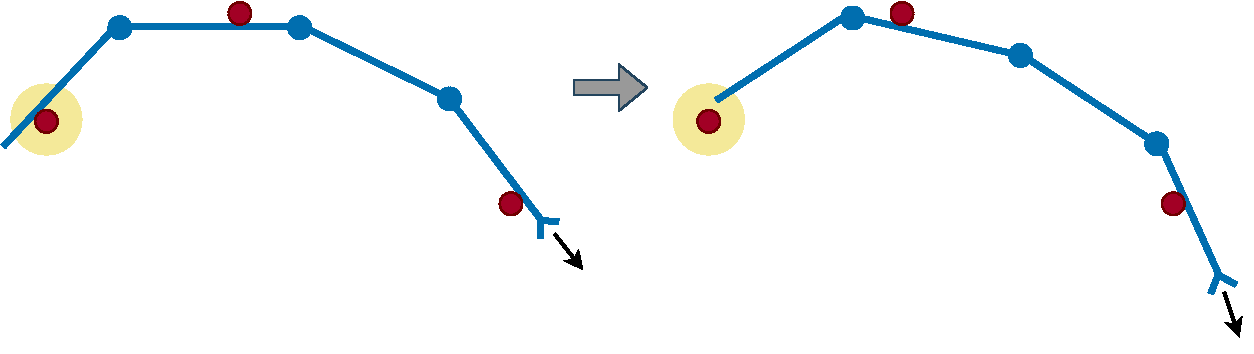
\includegraphics[width=\textwidth]{figures/theory/obst_slide_sequence1.pdf}
    \caption{Snake robot losing contact with obstacle}
    \label{fig:obst_slide_seq1}
\end{figure}

\begin{figure}[h!]
    \centering
    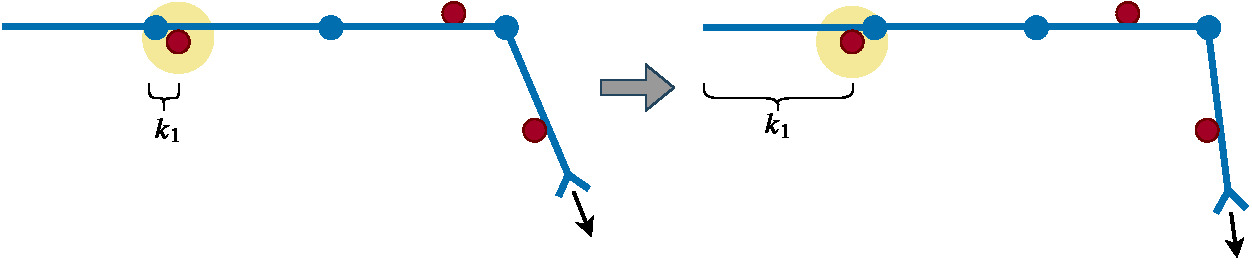
\includegraphics[width=\textwidth]{figures/theory/obst_slide_sequence2.pdf}
    \caption{Obstacle changing contact from one link to another}
    \label{fig:obst_slide_seq2}
\end{figure}

If, on the other hand, the snake simply slides in a way that the contact is transferred to an adjoining link, the size $n_c$ and dimensions of all variables will remain unchanged. In addition to this, the obstacle will lie on the same side of the snake as it already was, which enables the direction of the desired force application to the obstacle to stay the same. Thus, the constraint will generally be on the same form. The only thing that has to change is the description of the position variables in $\mathbf{r}_t$ belonging to the new contact point. Again, the change is most probably slim since the two first variables $(x_t, y_t)$ describe the position of the contact point, and the obstacle is assumed to be static (meaning its position will not change even though the calculation of the position changes). Furthermore, the adjoining link adopting the contact is probable to have a similar angle $\theta_t$ relative to the base frame as the previous link given that the desired path is well designed and defined. From this it follows that the joint variable $\phi_c$ back to the obstacle frame will stay similar to what it was as well. These aspects obviously make the implementation simpler and the control sequence smoother and more predictable.

Even though the numerical value of the mentioned variables do not change drastically, the Jacobian will have to be recalculated since the variables now are described by a new subset of the joint variables. Finding a new expression for the Jacobian matrix and its derivative in real-time is not a trivial, nor fast, operation. One option would of course be pre-computing $\mathbf{J}$ and $\dot{\mathbf{J}}$ for every link that could be in contact with an obstacle and only employ the ones that are relevant at the specific time instance. There is however still a challenge related to this case. The generalized joint variables $\mathbf{q}$ contain the distances $k$ from the contact points to the preceding joints. It is important that these distances are not mixed and that they are only used once. In other words, two contact points should not be described by the same $k$. As a consequence of this, the Jacobian for every link would have to be computed with all the possible $k$'s. Logically, this would in turn lead to a large number of pre-computed matrices as the number of links and obstacles grow. In addition to this, the right set of Jacobians would have to be chosen in real-time while administering that they all use unique $k$'s. This should be done without changing the existing setup more than necessary in order to avoid jumps in the control. It is very much an achievable task, but at the same time an extra challenge.

With a contact moving from one link to another, the corresponding joint variable $k$ describing the position of the contact point will change and the manner in which it is computed will also change. This is once again an achievable, yet challenging task to perform in real-time. It should also be noted that the value of this $k$ will probably experience a jump. This is because the contact moves from the end of a link to the beginning of a link, or vice versa, and the distance is always measured with respect to the preceding joint of the link in contact. This is illustrated in Figure \ref{fig:obst_slide_seq2}. On the other hand, it is reassuring that the matrices $\mathbf{M(q)}$ and $\mathbf{C(q,\dot{q})}$ are unaltered by the change of a $k$. This is logical since these matrices describe the dynamics of the snake robot alone.

The biggest challenge arises if the number of contact points increase. This means that the dimension of all variables will have to increase correspondingly and the Jacobians have to be either re-computed or re-assembled. It is in this case important to keep in mind the challenge associated with memory allocation in the software being used.

\subsection{Differences with the traditional manipulator case}

One significant challenge related to snake robots as opposed to traditional robot manipulators is the presence of passive joints at the base of the robot. The passive joints of the snake robot that are attached to the base frame, $[\phi_0, x_0, y_0]$ are included in the description of the position of every link and contact point. This means that if they were actuated, they could have influenced all the points that are desired to control, given that the robot is not stuck between obstacles. The dynamic hybrid position/force controller could therefore introduce a desired joint acceleration value $\ddot{\mathbf{q}}_d$ for these passive joints when recalculating from the desired contact point accelerations $\ddot{\mathbf{r}}_{t,d}$. Since these joints are passive, they are also uncontrollable and a desired control input on the joints is not realizable. A greater number of joints will generally make this challenge less significant because it leads to a larger degree of controllability of all contact points.

When it comes to the assignments of traditional robot manipulators and snake robots, they are usually a lot more repetitive and pre-defined for robot manipulators. A typical task for an industrial hybrid position force controlled robot manipulator is polishing a known surface with a given pressure. An example is given in Figure \ref{fig:robotman-polish}. The snake robot might also be familiar with the shape of its current environment, but this is something that is constantly changing as the robot moves through the world. Thus, the position and force application requirements are constantly changing as well. Furthermore, since the snake robot is eventually meant to locomote through outdoor environments, it will encounter different kinds of obstacles as illustrated in Figure \ref{fig:weird-env}. They can differ in both size and texture, and be either soft or rigid. Thus, there are a lot of factors the snake robot will have to take into account. For this project however, the environment and control goals are significantly simplified.

\begin{figure}
    \centering
    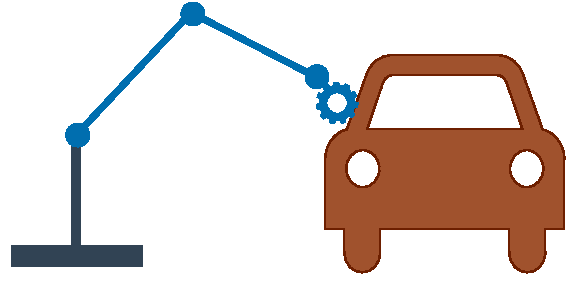
\includegraphics[width=0.6\textwidth]{figures/theory/robotman-polish.pdf}
    \caption{Industrial robot manipulator polishing a car}
    \label{fig:robotman-polish}
\end{figure}

\begin{figure}
    \centering
    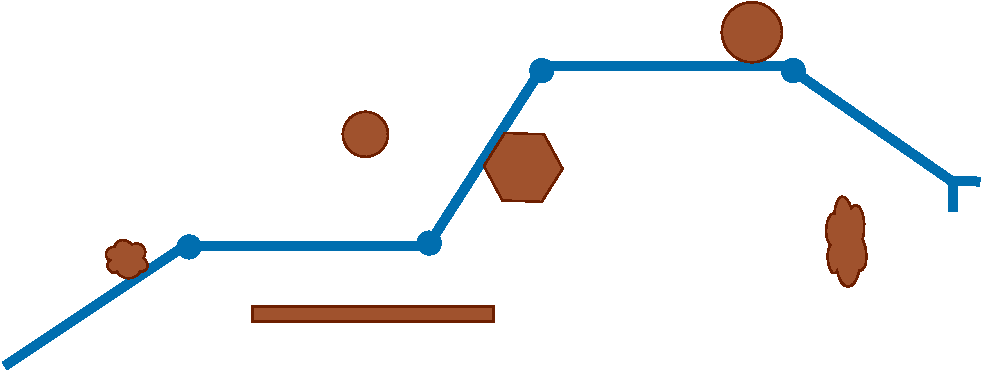
\includegraphics[width=0.7\textwidth]{figures/theory/weird-environment.pdf}
    \caption{Snake robot in environment with varying obstacle types}
    \label{fig:weird-env}
\end{figure}

There is also a considerable difference in the typical constraints on a snake robot and a traditional manipulator. Manipulators usually only have constraints or obstacles in the close environment of the end effector in which the manipulator is performing a task. It might also have some limitations regarding the motion span of its joints, but this applies to snake robots as well, though perhaps to a smaller degree. The environment the snake robot is traversing may as mentioned contain various and spread out obstacles, making the constraints different from time to time. If, however, a robot is in an undesirable position between obstacles, a snake robot might have an advantage in that it can exit its current configuration from several different directions since no part of it is fixed to any point in the world.

%- Arbitrary number of obstacles and constantly changing requirements (desired force application etc, as opposed to a typical industrial manipulator that simply should polish a surface with a given pressure repeatedly)

%- The environment is constantly changing and the contact wont be a point contact in the real world, and the snake robot might encounter all kinds of surfaces and textures (rigid, soft, slippery etc)
%%%%%%%%%%%%%%%%%%%%%%%%%%%%%%%%%%%%%%%%%%%%%%%%%%%%%%%%%%%%%%%%%%%%%%%%%%%%%%%%%%%%%%%%%%%%%
%%%%%%%%%%%%%%%%%%%%%%%%%%%%%%%%%%%%%%%%%%%%%%%%%%%%%%%%%%%%%%%%%%%%%%%%%%%%%%%%%%%%%%%%%%%%%


\subsection{Example of dynamic HPFC on simple snake robot}

This section shows a very simple scenario with a 2-link robot and one obstacle. The aim is to provide a better understanding of the theory presented in \ref{subsec:DHPFC} and show the structure of the various mapping matrices.
Furthermore, the example shows the necessity of using simulation software to study more intricate cases, as the matrices for this simple case already get quite complex.

The configuration of the robot and its environment is illustrated in Figure \ref{fig:ex_2link}. %To make the example as simple as possible, the robot is still in the given configuration and all velocities are thus zero.
The mass of each link is $m = 1 kg$ and the link length is $l=1 m$. The value of the joint angles $\phi_0$ and $\phi_1$ are $0$ and $\pi/2$ respectively.

\begin{figure}
    \centering
    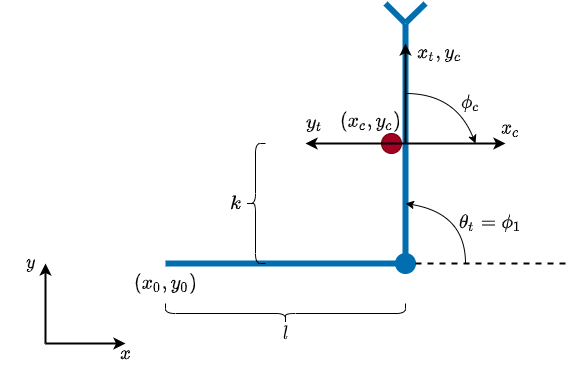
\includegraphics[width=0.9\textwidth]{figures/theory/example_2link.png}
    \caption{Model of 2-link snake robot}
    \label{fig:ex_2link}
\end{figure}

The joint variables are given by

\begin{equation}
    \mathbf{q} =
    \begin{bmatrix}
        \phi_0 & \phi_1 & x_0 & y_0 & k & \phi_c
    \end{bmatrix}^T \in \mathcal{R}^5.
\end{equation}
\\
The task coordinates by the contact point are given by

\begin{equation}
    \mathbf{r}_t = 
    \begin{bmatrix}
        x_c & y_c & \theta_t
    \end{bmatrix}^T \in \mathcal{R}^3,
\end{equation}
\\
where $\theta_t$ in the given configuration is the sum of the two joint angles $\phi_0$ and $\phi_1$. Furthermore, the constraint coordinates, which should always remain constant, are given by

\begin{equation}
    \mathbf{r}_c = 
    \begin{bmatrix}
        x_c & y_c & \theta_c
    \end{bmatrix}^T \in \mathcal{R}^3,
\end{equation}
\\
where $\theta_c$ is the angle of the obstacle point coordinate system in the base frame. This angle should always be zero, as can be seen from Figure \ref{fig:ex_2link}. It should be noted that the origin of the two frames, described by $(x_c, y_c)$, is the same. This is a result of the contact point and obstacle being modeled as a single point.

Lastly, the velocities and forces represented in the task frame (visualized in Figure \ref{fig:ex_2link} as $(x_t, y_t)$) are 

\begin{equation}
    \mathbf{v} =
    \begin{bmatrix}
        v_x & v_y
    \end{bmatrix}^T \in \mathcal{R}^2,
\end{equation}

\begin{equation}
    \mathbf{f} =
    \begin{bmatrix}
        f_x & f_y
    \end{bmatrix}^T \in \mathcal{R}^2.
\end{equation}
\\

\subsubsection{Dynamics}

The dynamics of this robot can be found using the Euler-Lagrange method described in \ref{sec:dyn}.
The position and velocities of the middle of the links in the base frame are

\begin{equation}
    \begin{split}
        p_0 &=
        \begin{bmatrix}
            x_0 + l/2 cos(\phi_0)\\
            y_0 + l/2 sin(\phi_0)
        \end{bmatrix}, \\
        p_1 &=
        \begin{bmatrix}
            x_0 + l cos(\phi_0) + l/2 cos(\phi_0+ \phi_1)\\
            y_0 + l sin(\phi_0) + l/2 sin(\phi_0+\phi_1)
        \end{bmatrix},
    \end{split}
\end{equation}

\begin{equation}
    \begin{split}
        \dot{p}_0 &=
        \begin{bmatrix}
            \dot{x_0} - l/2 \dot{\phi_0} sin(\phi_0)\\
            \dot{y_0} + l/2 \dot{\phi_0} cos(\phi_0)
        \end{bmatrix}, \\
        \dot{p}_1 &=
        \begin{bmatrix}
            \dot{x_0} - l \dot{\phi_0} sin(\phi_0) - l/2 (\dot{\phi}_0 +\dot{\phi}_1) sin(\phi_0+\phi_1)\\
            \dot{y_0} + l \dot{\phi_0} cos(\phi_0) + l/2 (\dot{\phi}_0 +\dot{\phi}_1) cos(\phi_0+\phi_1)
        \end{bmatrix}.
    \end{split}
\end{equation}
\\
The Lagrangian and the dynamical equations can now be calculated from (\ref{eq:ex_dyn1}) and (\ref{eq:ex_dyn2}), where $I = (1/12)ml^2 = 1/12$.

\begin{equation}\label{eq:ex_dyn1}
    \begin{split}
        L &= K_{translational,0} + K_{rotational,0} + K_{translational,1} + K_{rotational,1}\\
        &= \frac{1}{2} m \dot{p}_0^2 + \frac{1}{2}I\dot{\phi_0}^2 + \frac{1}{2} m \dot{p}_1^2 + \frac{1}{2}I\dot{\phi_1}^2
    \end{split}
\end{equation}
\\
\begin{equation}\label{eq:ex_dyn2}
    \boldsymbol{\tau} = \frac{d}{dt} \frac{\partial L}{\partial \dot{\mathbf{q}}} - \frac{\partial L}{\partial \mathbf{q}}
\end{equation}
\\
Inserting the values for the constants $m$ and $l$ and comparing the result to the form given in (\ref{eq:eom}) gives the inertia and Coriolis matrix in (\ref{eq:ex_inertia}) and (\ref{eq:ex_coriolis}) respectively. The trigonometric functions are abbreviated to $s_0 = sin(\phi_0)$, $s_1 = sin(\phi_1)$, $c_0 = cos(\phi_0)$, $c_1 = cos(\phi_1)$, $s_{01} = sin(\phi_0+\phi_1)$ and $c_{01} = cos(\phi_0+\phi_1)$.

\begin{equation}\label{eq:ex_inertia}
    \mathbf{M(q)} = 
    \begin{bmatrix}
        c_1+\frac{5}{3} & \frac{c_1}{2} + \frac{1}{3} & -\frac{s_{01}}{2} - \frac{3s_0}{2} & \frac{c_{01}}{2} + \frac{3c_0}{2} & 0 & 0 \\
        \frac{c_1}{2}+\frac{1}{3} & \frac{1}{3} & -\frac{s_{01}}{2} & \frac{c_{01}}{2} & 0 & 0 \\
        -\frac{s_{01}}{2}- \frac{3s_0}{2} & -\frac{s_{01}}{2} & 2 & 0 & 0 & 0 \\
        \frac{c_{01}}{2}+ \frac{3c_0}{2} & \frac{c_{01}}{2} & 0 & 2 & 0 & 0 \\
        0 & 0 & 0 & 0 & 0  & 0 \\
        0 & 0 & 0 & 0 & 0  & 0
    \end{bmatrix}
\end{equation}

\begin{equation}\label{eq:ex_coriolis}
    \mathbf{C(q, \dot{q})} = 
    \begin{bmatrix}
        -\frac{\dot{\phi}_1 s_1 (2\dot{\phi}_0+ \dot{\phi}_1)}{2} \\
        \frac{\dot{\phi}_0^2 s_1}{2} \\
        -\frac{3 \dot{\phi}_0^2 c_1}{2} - \frac{\dot{\phi}_0^2 c_{01}}{2} - \frac{\dot{\phi}_1^2 c_{01}}{2} - \dot{\phi}_0 \dot{\phi}_1 c_{01} \\
        -\frac{3 \dot{\phi}_0^2 s_1}{2} - \frac{\dot{\phi}_0^2 s_{01}}{2} - \frac{\dot{\phi}_1^2 s_{01}}{2} - \dot{\phi}_0 \dot{\phi}_1 s_{01} \\
        0 \\ 0
    \end{bmatrix}
\end{equation}
\\
Inserting the given angles significantly simplifies the matrices to

\begin{equation}
    \mathbf{M} = 
    \begin{bmatrix}
        5/3 & 1/3 & -1/2 & 3/2 & 0& 0 \\
        1/3 & 1/3 & -1/2 & 0 & 0 & 0\\
        -1/2 & -1/2 & 2 & 0 & 0 & 0\\
        3/2 & 0 & 0 & 2 & 0 & 0\\
        0 & 0 & 0 & 0 & 0 & 0\\
        0 & 0 & 0 & 0 & 0 & 0
    \end{bmatrix}
\end{equation}

\begin{equation}
    \mathbf{C(\dot{q})} = 
    \begin{bmatrix}
        -(\dot{\phi}_1 (2\dot{\phi}_0+ \dot{\phi}_1))/2 \\
        \dot{\phi}_0^2/2 \\
        0 \\
        -3 \dot{\phi}_0^2/2 - \dot{\phi}_0^2/2 - \dot{\phi}_1^2/2 - \dot{\phi}_0 \dot{\phi}_1 \\
        0 \\ 0
    \end{bmatrix}.
\end{equation}

\subsubsection{Constraints}

The single obstacle present in this example stands for the single constraint on the snake robot. 
From \ref{subsec:DHPFC} it is known that the constraint is on the velocity of the contact point normal to the link in contact. This velocity is here given as

\begin{equation}
    v_y = - sin(\theta_t) \dot{x}_c + cos(\theta_t) \dot{y}_c
\end{equation}
\\
In order for the link to both stick to the obstacle and not penetrate it, the velocity $v_y$ should be zero. This constraint is put on the form in (\ref{eq:hpfc:derhypsurf}) and the given angles are inserted.

\begin{equation}\label{eq:ex_EF}
    \mathbf{E}_F = 
    \begin{bmatrix}
        - sin(\theta_t) & cos(\theta_t) & 0
    \end{bmatrix}
    =
    \begin{bmatrix}
        - 1 & 0 & 0
    \end{bmatrix}
\end{equation}
\\
The derivative of (\ref{eq:ex_EF}) is
\begin{equation}\label{eq:ex_EFd}
    \mathbf{\dot{E}}_F = 
    \begin{bmatrix}
        -cos(\theta_t) \dot{\theta}_t & - sin(\theta_t) \dot{\theta}_t & 0
    \end{bmatrix}
    \begin{bmatrix}
        0 & -\dot{\theta}_t & 0
    \end{bmatrix}.
\end{equation}
\\
Inserting (\ref{eq:ex_EFd}) into (\ref{eq:dhpfc_arf}) gives
\begin{equation}
    a_{rF} = -\dot{\theta}_t \dot{y}_c.
\end{equation}
\\
It is however known that the obstacle itself cannot move. This, together with the obstacle being modeled as a point, results in the velocity of the contact point being zero at all times. Thus $a_{rF}=0$.

(\ref{eq:dhpfc_EPi}) and (\ref{eq:dhpfc_E}) give
\begin{equation}
    \mathbf{E}_P = 
    \begin{bmatrix}
        cos(\theta_t) & sin(\theta_t) & 0 \\
        0 & 0 & 1
    \end{bmatrix}=
    \begin{bmatrix}
        0 & 1 & 0 \\
        0 & 0 & 1
    \end{bmatrix},
\end{equation}
\begin{equation}
    \mathbf{E}=
    \begin{bmatrix}
        0 & 1 & 0 \\
        0 & 0 & 1 \\
        -1 & 0 & 0
    \end{bmatrix}.
\end{equation}
\\
The task coordinates can be expressed as
\begin{equation}
    \mathbf{r}_t =
    \begin{bmatrix}
        x_0 + l cos(\phi_0) + k cos(\phi_0+\phi_1)\\
        y_0 + l sin(\phi_0) + k sin(\phi_0+\phi_1)\\
        \phi_0+\phi_1
    \end{bmatrix}.
\end{equation}
\\
The corresponding Jacobian an its derivative can thus be calculated to
\begin{equation}
    \begin{split}
        \mathbf{J}_t&=
        \begin{bmatrix}
            -l s_0 - k s_{01} & - k s_{01} & 1 & 0 & c_{01} & 0 \\
            l c_0 + k c_{01} & k c_{01} & 0 & 1 & s_{01} & 0 \\
            1 & 1 & 0 & 0 & 0 & 0
        \end{bmatrix}\\&=
        \begin{bmatrix}
            - k & - k & 1 & 0 & 0 & 0 \\
            1 &0 & 0 & 1 & 1 & 0 \\
            1 & 1 & 0 & 0 & 0 & 0
        \end{bmatrix},
    \end{split}
\end{equation}
\begin{equation}\label{eq:ex_Jd}
    \begin{split}
        \mathbf{\dot{J}}_t&=
        \begin{bmatrix}
            - \dot{k} s_{01} -l \dot{\phi}_0c_0 -k c_{01}(\dot{\phi_0}+\dot{\phi_1}) & -\dot{k} s_{01}-k c_{01}(\dot{\phi_0}+\dot{\phi_1}) & 0 & 0 & -s_{01}(\dot{\phi_0}+\dot{\phi_1})  & 0\\
            \dot{k} c_{01} -l \dot{\phi}_0s_0 -k s_{01}(\dot{\phi_0}+\dot{\phi_1}) & \dot{k} c_{01}-k s_{01}(\dot{\phi_0}+\dot{\phi_1}) & 0 & 0 & c_{01}(\dot{\phi_0}+\dot{\phi_1}) & 0 \\
            0 & 0 & 0 & 0 & 0 & 0
        \end{bmatrix}\\&=
        \begin{bmatrix}
            - \dot{k} -\dot{\phi}_0 & -\dot{k} & 0 & 0 & -(\dot{\phi_0}+\dot{\phi_1}) & 0 \\
            -\dot{k}(\dot{\phi_0}+\dot{\phi_1}) & -\dot{k}(\dot{\phi_0}+\dot{\phi_1}) & 0 & 0 & 0 & 0\\
            0 & 0 & 0 & 0 & 0 & 0
        \end{bmatrix}.
    \end{split}
\end{equation}
\\
Inserting (\ref{eq:ex_Jd}) into (\ref{eq:dhpfc_aq}) gives
\begin{equation}
    \mathbf{a}_q =
    \begin{bmatrix}
            - (\dot{k} +\dot{\phi}_0)\dot{\phi}_0 -\dot{k} \dot{\phi}_1 -(\dot{\phi_0}+\dot{\phi_1})\dot{k} \\
            -\dot{k}(\dot{\phi_0}+\dot{\phi_1})\dot{\phi}_0 -\dot{k}(\dot{\phi_0}+\dot{\phi_1})\dot{\phi}_1 \\
            0
        \end{bmatrix}.
\end{equation}

\subsubsection{Calculation of the control torque}

All matrices necessary to derive the control torque are now defined. To make the calculation of the torque even simpler, the static case where all velocities are zero is considered. The result is calculated using (\ref{eq:dhpfc_tau_c})-(\ref{eq:dhpfc_qddd}) and a desired force $f_F = 1 N$ and desired acceleration $\ddot{\mathbf{r}}_d = [0, 0, 1 rad/s^2]^T$. \hl{Quite fast rotation and light force?}

\begin{equation}
    \mathbf{\ddot{q}}_d =
    \begin{bmatrix}
        0 & \frac{1}{5} & \frac{2}{5}\\
        0 & -\frac{1}{5} & \frac{3}{5}\\
        1 & 0 & k \\
        0 & \frac{2}{5} & -\frac{1}{5}\\
        0 & \frac{2}{5} & -\frac{1}{5} \\
        0 & 0 & 0
    \end{bmatrix}\left\{
    \begin{bmatrix}
        0 & 0 & -1\\
        1 & 0 & 0\\
        0 & 1 & 0
    \end{bmatrix}
    \begin{bmatrix}
        0\\   1\\   0
    \end{bmatrix}-
    \begin{bmatrix}
        0\\   0\\   0
    \end{bmatrix}\right\}=
    \begin{bmatrix}
        \frac{2}{5}\\
        \frac{3}{5}\\
        k \\
        -\frac{1}{5}\\
        -\frac{1}{5} \\
        0
    \end{bmatrix}
\end{equation}
\\
The distance $k$ from the joint to the obstacle is chosen to be $1/2 m$.
\begin{equation}
    \boldsymbol{\tau}_P = 
    \begin{bmatrix}
        5/3 & 1/3 & -1/2 & 3/2 & 0 & 0 \\
        1/3 & 1/3 & -1/2 & 0 & 0 & 0 \\
        -1/2 & -1/2 & 2 & 0 & 0 & 0 \\
        3/2 & 0 & 0 & 2 & 0 & 0 \\
        0 & 0 & 0 & 0 & 0  & 0\\
        0 & 0 & 0 & 0 & 0  & 0
    \end{bmatrix}
    \begin{bmatrix}
        2/5\\
        3/5\\
        k \\
        -1/5\\
        -1/5\\0
    \end{bmatrix}=
    \begin{bmatrix}
        0.3167\\
        0.0833\\
        0.5000 \\
        0.2000\\
        0\\0
    \end{bmatrix}
\end{equation}

\begin{equation}
    \boldsymbol{\tau}_F = 
    \begin{bmatrix}
       -k & 1 & 1\\
       -k & 0 & 1\\
       1 & 0 & 0\\
       0 & 1 & 0\\
       0 & 1 & 0 \\
       0 & 0 & 0
    \end{bmatrix}
    \begin{bmatrix}
        -1 \\ 0 \\ 0
    \end{bmatrix}=
    \begin{bmatrix}
       0.5000\\
       0.5000\\
       -1.000\\
       0.000\\
       0.000\\ 0
    \end{bmatrix}
\end{equation}

\begin{equation}
    \boldsymbol{\tau}_c =
    \begin{bmatrix}
        0.8167 & 0.5833 & -0.5000 & 0.2000 & 0.000 & 0.000
    \end{bmatrix}^T
\end{equation}

\hl{Discuss this result. The torques to the translational positions cannot be applied. Is this what the servo feedback thing is for?? only tau 1 can really be applied. k ends up being a free variable!}

%%%%%%%%%%%%%%%%%%%%%%%%%%%%%%%%%%%%%%%%%%%%%%%%%%%%%%%%%%%%%%%%%%%%%%%%%%%%%%%%%%%%%%%%%%%%%
%%%%%%%%%%%%%%%%%%%%%%%%%%%%%%%%%%%%%%%%%%%%%%%%%%%%%%%%%%%%%%%%%%%%%%%%%%%%%%%%%%%%%%%%%%%%%



%\section{Constraint space analysis}

%Constraints typisk bare på end effector på manipulatorer. Hvis de har constraints flere steder derimot som en slange har slangen en fordel at den kan komme seg "ut" fra flere vinkler --> end effector workspace er mye større når den kan utilize alt i verden til å dytte seg hit og dit og den kan krølle sammen halen.

%Constraint Jacobian vs task Jacobian.


\section{Task analysis}

Even though the control solution presented in \ref{subsec:DHPFC} decomposes the workspace in force and movement directions, there are some restrictions as to which tasks can be performed by the robot. To analyze this, it is beneficial to look at what kind of tasks a snake robot is required to achieve. In particular, the tasks of a snake robot moving according to the OAL principle will be covered in this section. Both a higher level path following goal and a lower level control goal is presented. It is the lower level goal that will be further investigated in this project, but it is still important to keep in mind what the final purpose of the snake robot is.

Lastly, the task restrictions are discussed, followed by a mathematical adaption of the control scheme in \ref{subsec:DHPFC} based on the theory of West and Asada \cite{west1985method} described in \ref{subseq:HPFC}. This adaption is constructed to allow for the control of the task-relevant variables in cases where all task space variables cannot be controlled independently.

\subsection{The overall task of the snake robot}

The motivation behind implementing the OAL principle on a snake robot is to make it move from one point in space to another by utilizing the obstacles present in its environment. In a "real world" situation, solely moving around is not enough and the snake robot will normally have some auxiliary assignment as well. This can typically be documenting its surroundings with a camera or similar equipment attached to its foremost link, referred to as its head. This again makes the snake robot's exact path from the starting point to the end point relevant, and the path following of the head of the snake robot is thus the overall goal. When a path has been designed, this goal can be decomposed in tasks consisting of the global position and orientation of the snake robot head. In traditional robot manipulator theory, this would be referred to as the end-effector movement. 


\subsection{Lower level control tasks}

Because the base of traditional manipulators are fixed to the ground, they can move the end effector in a desired manner simply by following the inverse kinematics. This is of course given that the robot's degrees of freedom satisfy the desired end effector movement. For snake robots, on the other hand, it is more complicated.
In order to reach the higher level path following goal, the snake robot has to push itself forward in a purposeful manner utilizing the obstacles in the environment. By purposeful it is meant that the direction of the force application against the obstacles have to conform with the desired propulsion direction given by the path. This is where the hybrid position force control comes into play. The robot has to both position itself in a certain manner alongside the obstacles and push against them with a given force magnitude.

The general idea is that at any point in time a task will be given by a higher level path following algorithm which is assumed implemented. The information provided should include which obstacles are to be utilized and how the snake robot is to utilize them. In other words, the tasks sent to the hybrid position/force controller simply consist of a desired positioning (orientation) by every obstacle and force to be applied to the obstacles.



\subsection{Task restrictions}\label{subsec:task-restrictions}

The question is, what are the restrictions to which tasks the higher level path following algorithm can command the snake robot to perform? It is obvious that not any given combination of position and force can be simultaneously achieved.

The restrictions lie in the composition of the snake robot, meaning how many joints the robot consists of. A higher number of joints, and thus actuators, enables the robot to control a higher number of variables. At the same time, a higher number of contact points imposes a higher number of constraints on the system and therefore limits the controllability. That is not to say that few contact points are desired, because they are after all a necessity for successful propulsion.

For every contact point there are three possible variables that can be controlled. In \ref{subsec:DHPFC} it is defined that two of these variables belong to the position control. That is the movement along the obstacle and rotation by or around the obstacle. The remaining variable is reserved for the force against the obstacle.

To analyze the restrictions to how many and which of these variables can be controlled for a given robot, it is useful to look at the robot's closed kinematic chains (CKCs). A kinematic chain is said to be closed when it contains one or more loops \cite{lynch2017modern}. In the snake robot case loops arise between points fixed in the world (base frame). These points are the base of the robot, meaning the start of the first virtual translational joint, and every obstacle contact point. This is always true since it is assumed that the position of the obstacles are fixed in the world.

The number of CKCs is the same as the number of contact points on the robot. However, they can be expressed in several different ways. The first method is to define all closed kinematic chains from the base to every contact point. This is depicted in Figure \ref{fig:CKC1}, where $b$ denotes the base and $r_{c,i}$ denotes the different contact points.

\begin{figure}[h!]
    \centering
    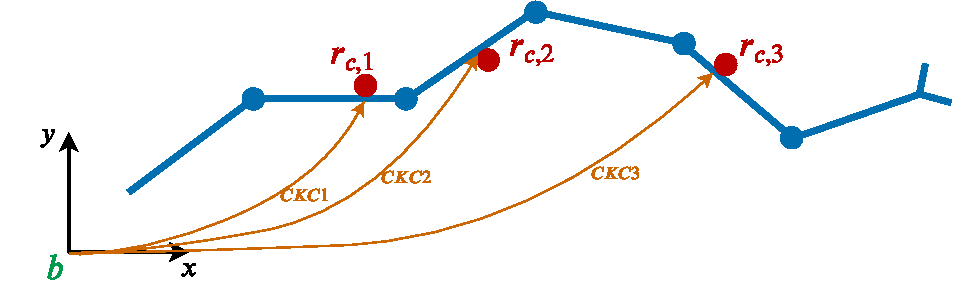
\includegraphics[width=0.9\textwidth]{figures/theory/CKC1.pdf}
    \caption{First method of defining the closed kinematic chains}
    \label{fig:CKC1}
\end{figure}

It is also possible to define the CKCs sequentially through the robot. Starting at the base again, the first CKC will be from the base to the first contact point. Moving further, the second chain will be from the first to the second contact point, then from the second to the third, etc. This definition of the CKCs is depicted in Figure \ref{fig:CKC2}, and will from now on be referred to as a minimal CKC representation. There are still many possible ways of defining the CKCs, but the two mentioned methods are the most relevant in this case.

\begin{figure}[h!]
    \centering
    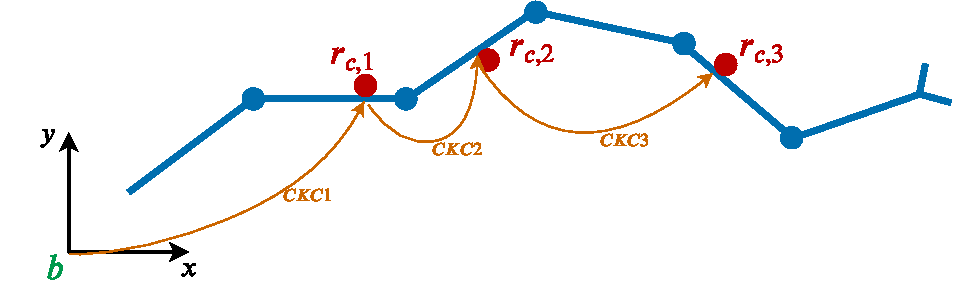
\includegraphics[width=0.9\textwidth]{figures/theory/CKC2.pdf}
    \caption{Second method of defining the closed kinematic chains}
    \label{fig:CKC2}
\end{figure}

The number of available actuators for controlling the variables at a single contact point are limited by the placement of the preceding contact point. This is because the CKC between these two points always is the smallest CKC with the least number of actuators and thus the so called bottleneck for the control.

To better explain this, the example snake robot illustrated in figures \ref{fig:CKC1} and \ref{fig:CKC2} is studied. In Figure \ref{fig:CKC1} there are four actuators included in the third CKC (CKC3) which is describing the third contact point. However, when looking at the closed kinematic chain for the same contact point described from its preceding contact point (depicted in Figure \ref{fig:CKC2}), only two actuators are included. Simply by studying the two figures it is also possible to see that the latter method always gives the minimal CKCs.

The ideal way of designing snake robots that require a high level of controllability is to include a very high number of joints. This way, even the minimal CKCs will have a sufficiently high number of actuators to make control at every contact point practically independent of the other contact points. Manipulators with such a large number of actuators are referred to as \textit{hyperredundant manipulators}. According to \cite{chiaverini2008kinematically}, a manipulator is considered to be hyperredundant if its controllable configuration space degrees of freedom are comparable to, or exceed, its task space degrees of freedom. Furthermore, it is stated that such manipulators have an enhanced potential to use their extra joints for maneuvering within tight obstacle fields. The term hyperredundant can be adapted to snake robots as well, and it is now obvious that hyperredundancy is a requirement for an ideal OAL-driven snake robot.

\subsubsection{Singularity avoidance}

A common problem when using Jacobian matrices for the inverse kinematic computations is the presence of singularities. A robot configuration $\mathbf{q}$ is singular if the task Jacobian matrix $\mathbf{J}_t$ is rank-deficient here \cite{chiaverini2008kinematically}. This configuration is not ideal since it means that it is impossible to generate task space velocities in certain directions. Task space velocities are for the snake robot velocities of the contact points vector $\mathbf{r}_t$. This is referred to as the end effector velocity in traditional robot manipulator theory.

An effect of a singularity is that the resulting joint space velocities can grow uncontrollably big. This effect is experienced not only at the singular configuration itself but also in its neighborhood \cite{chiaverini2008kinematically}. According to Chiaverini et al. \cite{chiaverini2008kinematically}, the distance to these singularities can be characterized through measurements based on the determinant of the Jacobian or the individual singular values of the matrix like the smallest singular value. If the snake robot consists of more joints than it needs for execution of the desired task, the additional degrees of freedom can be used to steer the snake robot away from singularities or avoid them at a planner level by analyzing these measurements. A more detailed description of the matter is presented in \cite{chiaverini2008kinematically}.
It should be noted that whether or not the robot is redundant depends both on the number of joints \textit{and} the number of contact points desired to control, i.e. the task.

Furthermore, the snake robot does not necessarily lose mobility in all task directions even though it is at a singular configuration. This is noteworthy since it might not be desirable for the snake robot to move in every possible direction anyway. In \ref{subsec:task-oriented} it is explained how the desirable or essential movement directions can be expressed and further utilized for control.


\subsection{Task oriented control scheme}\label{subsec:task-oriented}


In \ref{subseq:HPFC} it is stated that there are certain directions of force and movement that are essential for performing a task. It is further claimed that the number of essential directions can not be greater than the number of controllable actuators in the robot necessary for performing the task. In \ref{subsec:task-restrictions} it is explained that the number of available controllable actuators is limited by the minimal CKC.

For the snake robot, the force and movement directions of a task are described by $\mathbf{E}_F$ and $\mathbf{E}_P$.
%In some cases, the number of directions described by these vectors might exceed the number of active joints even though not all directions \textit{have} to be controlled precisely in order to perform the given task. So in other words, t
The number of essential directions in $\mathbf{E}_F$ and $\mathbf{E}_P$ together can not exceed the number of active joints in the minimal CKC. In the example in Figure \ref{fig:CKC2}, a maximum number of three variables at the second contact point could be desired to control. However, it is seen that the corresponding CKC only contains one actuator, meaning that at most one variable has to be chosen for control. In other words, the maximum number of essential variables that can be defined for performing a task at the second contact point is one.

As explained in \ref{subseq:HPFC}, the essential position and force directions can be described by (\ref{eq:hpfc_wep}) and (\ref{eq:hpfc_wef}). The filters (\ref{eq:hpfc_fp}) and (\ref{eq:hpfc_ff}) can then be used to focus the control on these essential directions, also taking into account which directions the robot is allowed to move and apply force in. This is of course given that the requirements regarding the number of active joints are fulfilled.

The force filter $\prescript{}{j}{\mathbf{F}}_{f}$, which is based on the allowable and essential force directions, can intuitively be combined with the input torque $\boldsymbol{\tau}_F$ for the desired force found by (\ref{eq:dhpfc_tauf}). It should be noted that the defined essential force directions and desired forces $\mathbf{f}_{F,d}$ have to correspond with each other. Combining the position filter $\prescript{}{j}{\mathbf{F}}_{p}$ with the position control torque from (\ref{eq:dhpfc_taup}) is unfortunately not as intuitive. This is because the filter is designed to map the joint velocities and not the joint torques. The dynamic HPFC control structure simply takes the desired contact point variables and directly computes the desired joint accelerations. This means that there is no intermediate step with joint velocities, as would have been convenient for the position filtering.

Under certain conditions and requirements, however, there are ways of combining the filter directly with the position control torque $\boldsymbol{\tau}_P$. First, it is known that as long as the position control is in fact performed in the position space, any acceleration $\ddot{\mathbf{q}}$ should lead to a change in velocity rather than force application. This again means there is a direct relationship between the joint accelerations and the velocities leading to the same "rules" being applicable for the two variables. Second, it is known that at very low velocities, the relationship between the joint torques and joint accelerations become approximately linear. This is because the moment of inertia of the links is constant in the used snake robot model. Again, it can be stated that the same rules apply for the position torque and desired position joint accelerations. Conclusively, the position filter $\prescript{}{j}{\mathbf{F}}_{p}$ can be used directly on the input torque for the desired position. It is again important that the essential position directions and desired position variables correspond.

Under the mentioned conditions, the new input control torques can be found by

\begin{equation}
    \boldsymbol{\tau}_c = \prescript{}{j}{\mathbf{F}}_{p} \boldsymbol{\tau}_P + \prescript{}{j}{\mathbf{F}}_{f} \boldsymbol{\tau}_F.
\end{equation}


\section{Hybrid obstacle aided locomotion (HOAL)}\label{sec:dhpfc-oal}

The motivation behind using dynamic HPFC for the OAL is that this locomotion method requires both interaction with the environment, meaning force application, and purposeful movement of the snake robot body. Instead of constantly switching between force and position control of the snake robot, the dynamic HPFC can manage to control both of these attributes simultaneously in different directions. Furthermore, the dynamic method is studied in this thesis because it is believed that the dynamics play an important role in the behavior of the snake robot and contribute to a dynamic rather than stiff control. This is even more significant in outdoor environments with friction, as opposed to a sterile, frictionless simulation environment. The downside is that modeling the friction and other traits of the environment becomes harder as the surroundings get more complex and diverse.

Being able to predict the dynamical response of the snake robot enables the feed forward control and thus a smoother control trajectory. 
The dynamics of going from no contact to contact have not been modeled in this project, and is believed to be a very complex task. It is yet to be assessed whether or not the collision-modeling can profit the overall control of the snake robot at all.

This section does not give any definite answers to how the HOAL scheme can be implemented. It does however discuss related challenges and provides some suggestions as to how the problem can be approached.

\subsection{General strategy for HOAL}

There is much more to HOAL than just pushing against obstacles and changing the shape of the robot at the same time. The snake robot needs an end goal, or at least a temporary goal to follow. The approach for reaching this goal should be assisted by a defined path from the current location of the snake robot. This path should be designed not only to allow the snake robot to pass by constructive obstacles for propulsion, but also to make it propel itself forward in the best way possible from start to finish. The best way is here considered to be a path that is both minimizing the distance and the energy usage. These attributes are of course not independent of each other.

%\cite{holden2014optimal} designed an optimization problem that seeks to minimize energy consumption while achieving propulsion along the desired path and thus determining the optimal use of the motor torques. Using this method requires the path to already be designed. It can however be discussed if the task of finding a desired path and the task of finding the optimal motor torques should be linked. For simplicity, they are kept separated for now.

A suggestion to a general procedure for achieving HOAL is given below

\begin{enumerate}
    \item Establish the position of the end goal of the snake robot head.
    \item Design a path from the current location of the snake robot to the end goal. Here, the distance should be minimized while taking into account that enough obstacles have to be passed by to achieve propulsion. The orientation of the robot along these obstacles should be taken into account as well.
    \item Determine the desired force magnitudes against each obstacle based on the desired propulsion speed of the snake robot head.
    \item Use dynamic HPFC and a suitable control structure to realize the desired forces and position/orientation defined by the steps above.
\end{enumerate}

\subsection{Conditions for propulsion}\label{subsec:prop-conditions}

There are some criteria that have to be fulfilled in order for the HOAL algorithm to be successful. First, it requires knowledge of the environment and the position of the obstacles within a given relevant range. Second, as mentioned earlier, the modeling of the dynamics should be as accurate as possible.

It is also relevant to look at the position and force spaces of the robot. In which direction is the snake robot actually able to apply forces? In which directions can it move freely? In which directions will movement lead to forward propulsion? In what configurations will the snake robot be jammed? These are all very important questions that should be addressed in the construction of the desired path.

According to Stavdahl \cite{StavdahlNote}, the position or motion space $\mathbb{M}$ can be decomposed into a shape space $\mathbb{S}$ and a propulsion space $\mathbb{P}$. Furthermore, the force space $\mathbb{F}$ is referred to as the constraint space $\mathbb{C}$ because it does not directly yield propulsion. The knowledge about these spaces can be utilized to design a path and a set of desired forces that support the snake robot in propelling itself forward.
%The most vital task is finding in which configurations the propulsion space of the robot is nonempty, as this is logically a necessary condition for propulsion. More specifically, it is desired to look at the individual non-singular directions, as the snake robot is meant to follow a given directed path and thus all directions are not relevant.
%When a path has been constructed, the constraint and shape spaces should be utilized to keep the snake robot head within its propulsion space. $\mathbb{C}$ can be used to keep the snake robot from getting jammed between obstacles. It should also be used to make sure the snake robot has a steady contact with all obstacles necessary. Furthermore, $\mathbb{S}$ is the remaining dimensions that can be used to change the shape of the robot according to the path. Thus, staying in the propulsion space is a necessary condition for propulsion, whereas the constraint and shape spaces make out the sufficient conditions that profit the necessary condition. \hl{mhm?? naah?}

%The issue that now has to be addressed is decomposing the motion space into $\mathbb{S}$ and $\mathbb{P}$.
In \ref{subseq:HPFC} it is shown how the allowable motion and force spaces can be deduced from the constraint Jacobian $\mathbf{J}_c$. Based on the same logic, the Jacobian $\mathbf{J}_P$ relating the joint velocities to the desired velocity of the snake robot head along the given path can be used to find the propulsion space. The pseudoinverse $\mathbf{J}^+_P$ can be used to find the joint velocities related to a given snake robot head velocity $\mathbf{v}_P$. The relation is given in (\ref{eq:endeff-vel}).

\begin{equation}\label{eq:endeff-vel}
    \dot{\mathbf{q}} = \mathbf{J}^+_P \mathbf{v}_P
\end{equation}
\\
Furthermore, $(\mathbf{I} - \mathbf{J}^+_P \mathbf{J}_P)$ represents the orthogonal projection matrix in the null space of $\mathbf{J}_P$ \cite{chiaverini2008kinematically}. That means that joint velocities projected onto this space yield zero velocity for the snake robot head. The shape space $\mathbb{S}$ can now be found as the remaining part of the motion space $\mathbb{M}$ that is not spanned by $\mathbb{P}$.

For propulsion it is not desired that the snake robot head is moved in an arbitrary direction, but rather in a specific direction defined by the desired path. Therefore, a necessary condition for propulsion will be that this particular direction is within the span of the propulsion space. Finding the general criteria for when this is satisfied still remains to be answered.

%In order to analyze the criteria for propulsion it is also relevant to look at the contact with the environment.
According to Bayraktaroglu \cite{bayraktaroglu2004understanding} a necessary condition for propulsion in a push-point-based locomotion approach is that the snake robot is in contact with and can push against at least three obstacles simultaneously. Bayraktaroglu \cite{bayraktaroglu2004understanding} further states that the total exterior forces and moments applied to a system must overcome the inertia and compensate perturbations in order to make it move with respect to a fixed reference frame. From this it follows that the directions in which the snake robot pushes against the obstacles is vital. To visualize this, two examples are presented. The first one is given in Figure \ref{fig:force-noprop}, in which it is obvious that no forward motion can be obtained from the resulting contact forces and the configuration is thus in the constraint space $\mathbb{C}$.

In Figure \ref{fig:force-prop} however, one of the links is able to push against an obstacle with a force $f_3$ that has a component in the forward (right) direction, enabling the snake robot to slide along the obstacle. This means that the propulsion space $\mathbb{P}$ is non-empty. The two other forces $f_1$ and $f_2$ contribute to keeping the end part of the snake in line. Additionally, they can be regarded as a kind of base for the snake robot to push against. If they were not included, the attempt to push against the third obstacle would only lead to a change of the snake robot's shape, meaning the configuration would be in the shape space $\mathbb{S}$. 

\begin{figure}[h!]
    \centering
    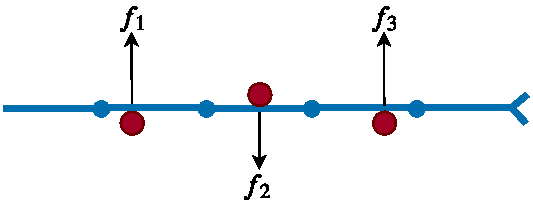
\includegraphics[width=0.6\textwidth]{figures/theory/obst-push-noprop.pdf}
    \caption{Force application yielding no propulsion}
    \label{fig:force-noprop}
\end{figure}

\begin{figure}[h!]
    \centering
    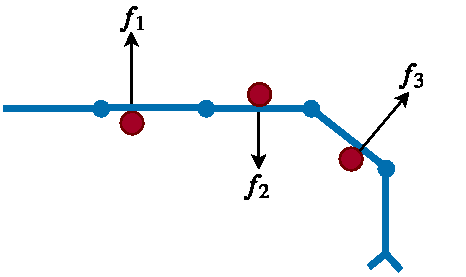
\includegraphics[width=0.5\textwidth]{figures/theory/obst-push-prop.pdf}
    \caption{Force application yielding propulsion}
    \label{fig:force-prop}
\end{figure}


The last example presenting forward propulsion does not include a desired trajectory for the snake robot to follow. Certain criteria will have to be met in the generation of the trajectory as well, and will typically be based on the composition of the snake robot. If the links are very long the snake robot will naturally not be able to shape itself along a very tightly curved path. If, on the other hand, the link length approaches zero the snake robot will resemble a natural snake and the limitations to its shape will decrease significantly. This type of robot is also referred to as a continuum robot, which according to Robinson et al. \cite{robinson1999continuum} is a continuously bending, infinite-degree-of-freedom structure. The goal in HOAL is not to adapt the snake robot composition to fit the path, but rather the path to fit the snake robot.

Figure \ref{fig:path-following} shows one case in which the curves of the desired path are sufficiently large for the snake robot to follow and one case in which the snake robot is physically unable to adjust itself perfectly to the desired path. The obstacles necessary for propulsion are left out in the illustrations.

\begin{figure}[H]
    \centering

    \subfloat[Successful path adjustment]{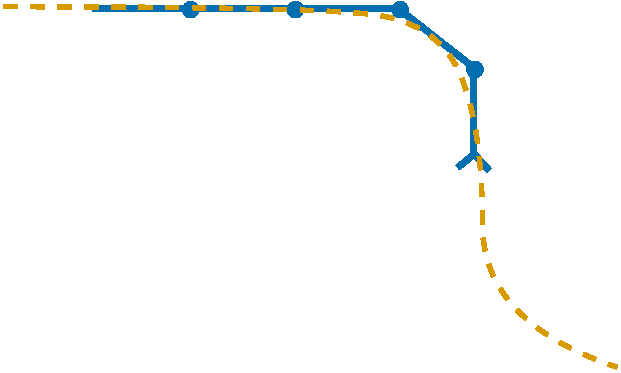
\includegraphics[width=0.5\textwidth]{figures/theory/path1.pdf}}
    \hfil
    \subfloat[Unsuccessful path adjustment]{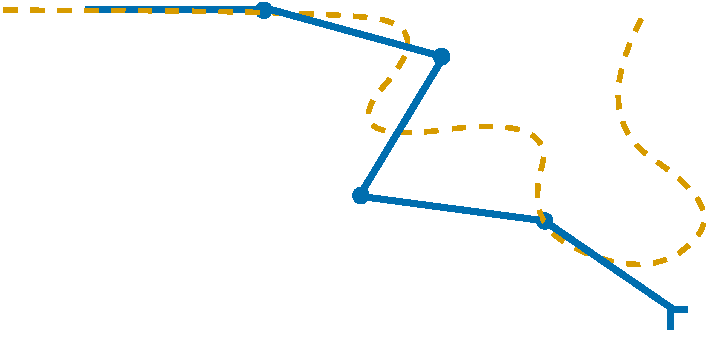
\includegraphics[width=0.5\textwidth]{figures/theory/path2.pdf}}

    \caption{Snake robot desired path following}
    \label{fig:path-following}
\end{figure}

It is clear that a distinct set of conditions for the desired path should be determined before the path planner is implemented. One hypothesis suggested by Stavdahl \cite{StavdahlNote} is that if the path consists of straight lines and circle segments, the radius of the circle segments have to be at least the same length as the snake robot link. The resulting curvature can be defined through the osculating circle, which is the circle that best approximates the curve at a point \cite{kline1998calculus}. The radius of this circle is denoted $r$, and the upper limit for the curvature is given by

\begin{equation}
    \kappa_{max} \leq \frac{1}{r_{min}} = \frac{1}{L}.
\end{equation}